%gives the problem structure used in the design of our
%numerical solution method. 
%Specifically, we design a 
%(PGD) %prox gradient 
%method 
%for solving this problem (see Section \ref{sec:pgd}). For this we must show that the function $u_\emu$
%is continuously differentiable with Lipschitz continuous gradient. 

%\section{Prox Gradient Descent}
\subsection{Proximal Gradient Descent for \texorpdfstring{$\uemu\tbg + R\tbg+\del_{\Rqp}(\tgam)$}{}} 
\label{sec:pgd}

We follow the analysis of the PGD algorithm given in \cite[Chapter 10]{AB17}
as it applies to the objective
%The application of the (PGD) %proximal gradient descent 
%algorithm to 
\begin{equation}\label{eq:varphi}
\Phi_\emu\tbg:=\uemu\tbg +\tR\tbg,\ \ \text{where}\ 
\tR\tbg:=R\tbg+\del_{\Rqp}(\tgam).
\end{equation}
%
%We now state the (PGD) %prox gradient descent 
%algorithm for finding a minimum for \eqref{eq:relax3}. 
Since $u_\emu$ is nonconvex, one typically 
applies a line search method to select stepsize. 
However, this is often not required in practice. 
For this reason we state the algorithm with and without a line search.
\medskip

%, as outlined in Algorithms \ref{alg:pgd_for_lme} and \ref{alg:MSR3}. 
%Set $\hR\tbg=R\tbg+\del_{\R^q_+}(\tgam)$ and 
%$\phi\tbg:=u_\emu\tbg+\hR\tbg$.
%See also Appendix 
%\smallskip

%\noindent
%{\bf Algorithm 1:} Proximal Gradient Descent with fixed stepsize (PGD)


%\noindent
%{\bf Algorithm 2:} Proximal Gradient Descent with Backtracking (PGD-B)

\begin{algorithm}[ht]
\SetAlgoLined
{\bf Initialize:} 
$\theta\in(0,1),\ \tau\in(0,1)$,
$\eta>0,\ \mu>0$, $\eps_{\mbox{\tiny Tol}}\ge 0$
$k=0$, $t_0>0$, $\bw^{0}=(\tbeta^0,\tgam^0)\in \Rp\times\R^q_+$
with $\inf\Phi_\emu <\Phi_\emu(\bw^0)$, 
$\gammax>\tgam^0$, 
$w^0=\prox_{t_0\tR}(\bw^{0}-t_0\nabla u_\emu(\bw^0))$.
%$, \ \eta_{Tol}\ge\eta_0>0,\ \mu_0\ge \mu_{Tol}>0$.
\\
\While{{\small $\norm{w^k-\bw^k}>\eps_{\mbox{\tiny Tol}}$
and $\gam^k\le\gammax$}}{\small\smallskip
\begin{enumerate}
\item[(i)] $t_{k+1}=\max\lset{t}{
\begin{aligned}&s\in\bW,\, t=t_0\theta^s,\ 
w=\prox_{t\tR}(w^k-t\nabla u_\emu(w^k))\\ &
\phi(w)
\le \phi(w^k)-\tau t\norm{w^k-w}^2
\end{aligned}}$.
\item[(ii)] $\bw^{k+1}=w^{k}$
\item[]$w^{k+1}=\prox_{t_{k+1}\tR}(w^k-t_{k+1}\nabla u_\emu(w^k))$
\item[]$k=k+1$
\end{enumerate}
}
\smallskip
\caption{\label{alg:pgd with bt}Proximal Gradient Descent 
fo $\Phi_\emu$ with Backtracking}
\end{algorithm}
\medskip


In Algorithm \ref{alg:MSR3}, 
the parameter $L$ is assumed to be a global Lipschitz
constant for $\nabla \uemu$. In Section \ref{sec:convergence pgd}, we show that the existence of $L$ is not needed.
In both algorithms we introduce the requirement that $\gam^k\le\gammax$.
While it is possible to include an explicit constraint of this form in the 
optimal variable selection problem \eqref{eq:lme_loss_original_in_x}, 
we do not do so since we assume that $\gammax$ is chosen 
so large that, from a practical perspective, 
the violation of this constraint indicates that the model is 
poorly posed and the algorithm needs to be terminated.
We base our analysis of the convergence properties of
Algorithms 1 and 2 on \cite[Theorem 10.15]{AB17} which makes use
of the following three basic assumptions:
\smallskip

\noindent
{\bf Basic Assumptions for the PGD Algorithm}
\begin{enumerate}
\item[(A)] $\map{\tR}{\Rp\times\Rq}{\eR}$ is a closed proper convex function.
\item[(B)] $\map{\uemu}{\Rp\times\Rq}{\eR}$ is closed and proper, 
$\dom{\uemu}$ is
convex, $\dom{\tR}\subset\intr{\dom{\uemu}}$, and
$\uemu$ is $L_\emu$-smooth over $\intr{\dom{\uemu}}$.
\item[(C)] Problem \eqref{eq:relax3} has an optimal solution with optimal 
value $\Phi_{\mbox{\tiny OPT}}$.
\end{enumerate}

\noindent
We assume that (A) holds. This is not an overly
restrictive assumption since it is satisfied by most of the standard
variable selection regularizers.
We show that (C) holds when $R$ satisfies
an additional coercivity hypothesis (Theorem \ref{thm:relaxed existence}). 
On the other hand, establishing that (B) holds
in a concrete setting such as ours
can be quite difficult. 
In particular, just as with $\LL$, $\uemu$ may fail to be globally Lipschitz.
Validating Assumption (B) as well as developing a technique for circumventing
the need for a global Lipschitz constant for $\nabla\uemu$ 
consumes the majority of the theoretical development. 
%Assumption (B) is particularly difficult since $\uemu$ is an optimal value function.
%We establish $B$ established in several steps.
%However, we show that the global Lipschitz continuity of $\nabla \uemu$
%is not required in practice for the theory developed in 
%\cite{AB17} to apply. 
%We begin by establishing the smoothness of $\uemu$.

%\begin{figure}[ht]
%    \centering
%    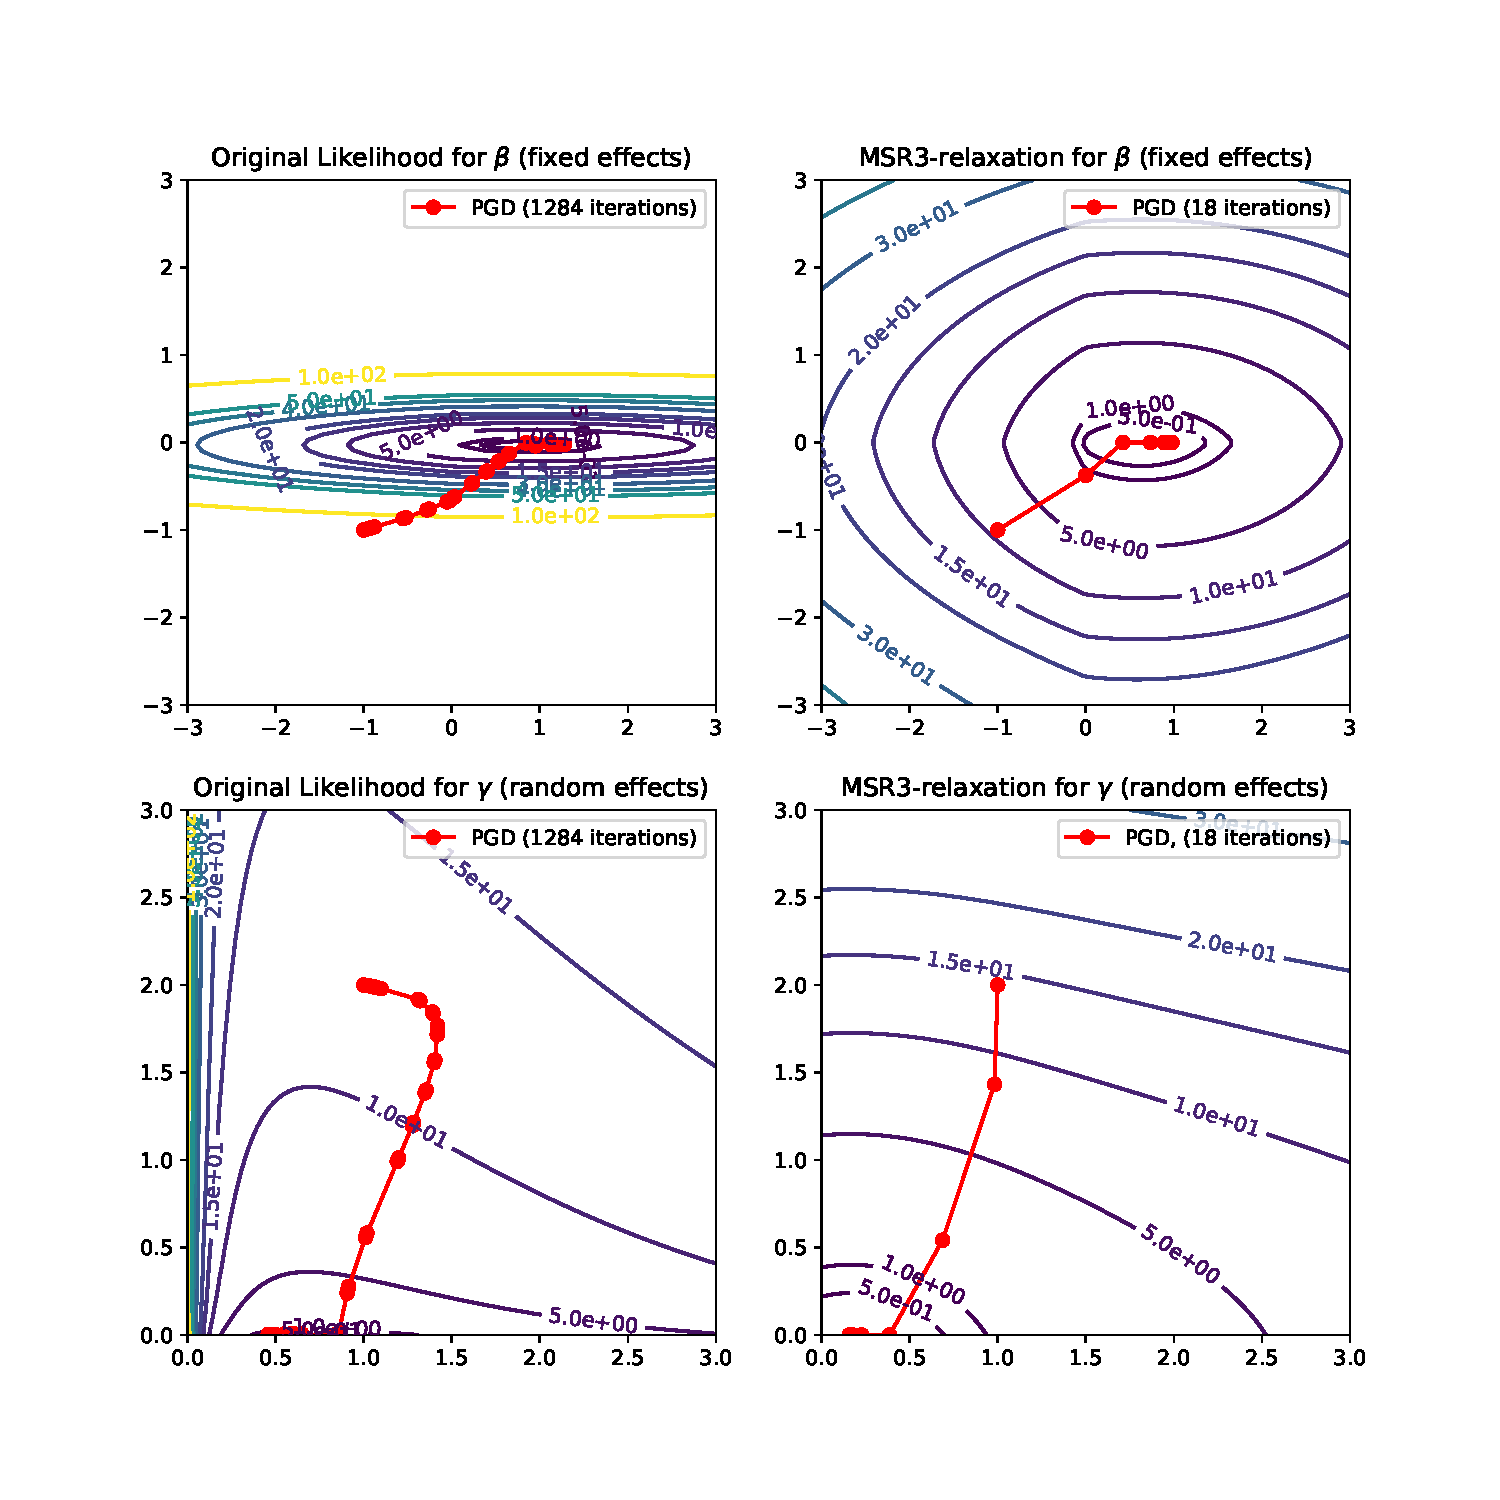
\includegraphics[width=\textwidth]{Images/intuition_current.pdf}
%    \caption{Proximal Gradient Descent (PGD) takes an order of magnitude fewer iterations to converge when optimizing a value function instead of the original likelihood, because SR3-relaxation improves the conditioning of the problem, which results in a more spherical level-sets. This effect persists for both quadratic convex (first row) and non-convex components (second row) of the likelihood. The effect is stronger for  minima near the boundary of the constraint region 
%    (bottom-left panel).}
%    \label{fig:geometric_intuition_sr3}
%\end{figure}


\subsection{The Smoothness of \texorpdfstring{$u_\emu$}{}}\label{sec:smoothness}
We investigate the relationship between the problems \eqref{eq:lme_loss_original_in_x}
and \eqref{eq:relax2}, the existence of solutions to 
 \eqref{eq:relax2}, and the properties of the function $\uemu$ and its derivative.
%We begin with an examination of the function $\LL$
%and 
%The first step is to understand the role of the parameter $\blam$.

\subsubsection{Underlying convexity}

\begin{lemma}[$\LL+\phimu$ is Weakly Convex]\label{lem:LL weak cvx}
Let $\LL$ be as given in \eqref{eq:lme_diagonal_setup}. Then
\begin{equation}\label{eq:hess LL}
\nabla^2\LL{(\beta,\gam)}=\sum_{i=1}^m
S_i^T\begin{bmatrix}X_i^T\\ -Z_i^T\end{bmatrix}
\Omega_i(\gam)^{-1}
\begin{bmatrix}X_i& -Z_i\end{bmatrix}S_i
-\begin{bmatrix}
0&0\\ 0& \half(Z_i^T\Omega_i(\gam)^{-1}Z_i)^{\circ2}
\end{bmatrix},
\end{equation}
for all
$(\beta,\gam)\in\R^p\times\R^q_+$, where 
\[
S_i:=\begin{bmatrix}
I_q&0\\ 0&\Diag{Z_i^T\Omega_i^{-1}(X_i\beta-Y_i)}
\end{bmatrix}
\]
and, for any $A\in\R^{t\times t}$, $A^{\circ 2}:=A\circ A$. In particular, this implies
that the matrix
\begin{equation}\label{eq:psd for LL}
\begin{bmatrix}
\nabla_{\beta\beta}\LL(\beta,\gam)&\nabla_{\gam\beta}\LL(\beta,\gam)\\
\nabla_{\beta\gam}\LL(\beta,\gam)&\nabla_{\gam\gam}\LL(\beta,\gam)
+\blam I\end{bmatrix}
\end{equation}
is positive semidefinite
for $\bar\eta= \nu m$, where
\[
\nu:=max\lset{(1/2) \mu_\mmin(\Lam_i)^{-2}\sig^4_\mmax(Z_i)}{i=1,\dots,m},
\]
$\mu_\mmin(\Lam_i)$ is the smallest eigenvalue of $\Lam_i$, and
 $\sig_\mmax(Z_i)$ is the largest singular value of $Z_i,\, i=1,\dots,m$.
Consequently, for any $\tbg\in\dom{\tR}$ and $\mu\ge 0$, the mapping 
\(
\bg\mapsto \LL_{\emu}(\bg, \tbg)
%\hLL(\bg,\tgam) %:=\LL(\beta,\gam)+\frac{\blam}{2}\norm{\gam-\hgam}^2
%\sum_{i=1}^m\frac{\nu_i}{2}\norm{\gam-\hat\gam}^2,
\)
is convex for all $\eta\ge\bar\eta:=\nu m$.
In particular, this implies that $\LL+\phimu$ is weakly convex for any $\mu\ge 0$, 
and the mapping
\(
%\begin{aligned}
\bg\mapsto\LL_{\emu}(\bg,\tbg)
%&=
%\LL\bg+\phimu(\gam)+
%\keta(\beta-\tbeta,\beta-\tbeta)
%\\ &=
%\hLL(\bg,\tgam)+    \frac{\eta}{2}\norm{\bg-\tbg}^2 
%\end{aligned}
\)
is strongly convex for $\eta> \bar\eta$ with modulus of strong convexity $(\eta-\bar\eta)$
regardless of the choice of $\tbg\in\Rp\times\Rq$.
%Moreover, the mapping 
%\eq{\label{eq:defn L sub eta}
%(\beta, \gamma)\mapsto    
%\LL_{\eta}(x, w) := \tLL(x, w) + \frac{\eta}{2}\norm{x-w}^2 
%}
%is strongly convex for every $\eta>0$ and any choice of 
%$(\tbeta,\tgam)\in\R^p\times\R^q$.
\end{lemma}
\begin{proof}
The formula for $\nabla^2\LL$ is given in Appendix \ref{appendix:derivatives_of_lmm}
(see \eqref{eq:hess LL}).
By \cite[Theorem 3.1]{ABBP2021}, 
$\mu_\mmax(\left(Z_i^T\Omega_i(\gam)^{-1}Z\right)\le
\lam_\mmin^{-1}\sig_\mmax^2(Z_i)$, and since 
$\mu_\mmax(H^{\circ 2})\le \mu_\mmax^2(H)$
for all $H\in\bS^q_+$ \cite{HJ85}, we have
\[
\mu_\mmax\left(\half(Z_i^T\Omega_i(\gam)^{-1}Z_i)^{\circ2}\right)
\le (1/2) \lam_\mmin^{-2}
\sig^4_\mmax(Z_i)=:\nu_i
\qquad  i=1,\dots,m.
\]
This establishes that the matrix in \eqref{eq:psd for LL} is positive semidefinite.
Since $\phimu$ is convex, the mapping
\[
(\beta,\gam)\mapsto \LL_{\emu}(\bg,\tbg) %\hLL((\beta,\gam),\tgam)
\]
is strongly convex for any choice
of $\blam> \nu m$, where 
\eq{\label{eq:nu}
\nu:=\max_{i=1,\dots,m}\nu_i.
}
%The strong convexity statement follows from 
%the fact that
%$\nabla^2 \LL_{\eta}((\beta, \gamma), (\tbeta, \tgamma))
%=\nabla^2 \LL(\beta,\gam)+\eta I$ where $\nabla^2 \tLL(\beta,\gam)$
%is positive semidfinite.
\end{proof}
For the remainder of the paper, we assume that 
\eq{\label{eq:blam1}\eta> \nu m=:\bar\eta} 
so that the mapping
$(\beta,\gam)\mapsto \LL_{\emu}(\bg,\tbg)$ %\hLL((\beta,\gam),\tgam)$
is strongly convex with 
%$\nabla_{\bg\bg}^2\hLL(\bg,\tgam)$ 
positive definite Hessian
regardless of the 
choice of $\tgam\in\R^q$. With this in mind, the function $\uemu$ defined by
\eqref{eq:value_function_definition} resembles a Moreau envelope.
%of the convex function $\hLL+\phi_\mu$.
However, this is misleading since, in particular,
we are not even assured of the existence of solutions to
the optimization problem defining $\uemu$. 

\subsubsection{Existence and consistency}\label{ssec:existence and consistency}

To establish the existence of solutions to the relaxed
optimization problems \eqref{eq:relax2} and the
problems defining the parametrized family $\uemu$ in
\eqref{eq:value_function_definition}, we assume that $R$ is $1$-coercive.
\begin{lemma}\label{lem:lb plus 1c}
Given $\mu>0$ let $\phimu$ be as defined above, and assume that 
$\map{R}{\Rp\times\Rq}{\R\cup\{+\infty\}}$
is 1-coercive, i.e., 
\(
\liminf_{\Vert{\tbg}\Vert\rightarrow\infty}\Vert{\tbg}\Vert^{-1}R\tbg>0.
\)
Then 
%the objective function in \eqref{eq:relax},
$\phimu+R$ 
%\(
%\wLL_\emu(\bg,\tbg):=\LL_{\emu}(\bg, \tbg)+R\tbg+\del_{R^q_+}(\tgam)
%\),
is level compact.
\end{lemma}
%\begin{proof}
%By Lemma \ref{lem:LL weak cvx}, for every $\tbg \in\Rp\times\Rq$,
%the mapping 
%$\bg\mapsto \LL_{\emu}(\bg, \tbg)$
%is strongly convex with modulus of strong convexity $\eta$.
%Consequently, for every $\tbg \in\Rp\times\Rq$,
%\[
%\begin{aligned}
%\LL_{\emu}((0,\one),\tbg)&+
%\ip{\nabla_{\bg}\LL_{\emu}((0,\one),\tbg)}{\bg-(0,\one)}+
%\frac{\eta}{2}\norm{\bg-(0,\one)}^2
%\\
%&\le \LL_{\emu}(\bg, \tbg)
%\qquad\forall\, \bg\in\Rp\times\R^q_{++},
%\end{aligned}
%\]
%which implies that
%\[\begin{aligned}
%&\LL(0,\one)+q\mu\ln(\mu)+\kappa_\eta(\tbeta,\tgam-\one)
%-\norm{\nabla_\beta \LL(0,\one)}\norm{\beta}-
%\norm{\nabla_\gam \LL(0,\one)}\norm{\gam-\one}-\mu^2\sqrt{q}\norm{\gam-\one}
%\\ &
%-\eta\ip{\tbeta}{\beta}+(\blam+\eta)\ip{\one-\tgam}{\gam-\one}
%+\frac{\eta}{2}\norm{(\beta,\gam)-(0,\one)}^2
%\\ &
%\le \LL_{\emu}(\bg, \tbg)
%\qquad\qquad\forall\, \bg\in\Rp\times\R^q_{++}.
%\end{aligned}
%\]
%That is, there are constants $\xi_0\in\R,\ \xi_1,\xi_2,\xi_3,\xi_4>0$ such that
%\[
%\begin{aligned}
%\xi_0+(\xi_2\norm{\beta}^2-\xi_1\norm{\beta})
%+(\xi_4\norm{\gam-1}^2-\xi_3\norm{\gam-\one})
%-\eta\ip{\tbeta}{\beta-\tbeta}-(\blam+\eta)\ip{\one-\tgam}{\gam-\one}
%\\ 
%\leq\LL_{\emu}(\bg, \tbg)
%\quad\forall\, \bg\in\Rp\times\R^q_{++}.
%\end{aligned}
%\]
%\end{proof}
%
\begin{proof}
If $\mu=0$, then the result is trivially true, so we assume that $\mu>0$.
Let $\{\bgk\}\subset \Rp\times\Rqp$ be such that $\norm{\bgk}\uparrow\infty$.
We need to show that $\phimu(\gam^k)+R\bgk\rightarrow \infty$.
If $\{\gam^k\}$ is bounded, then $\phimu(\gam^k)+R\bgk\rightarrow \infty$
since in this case $\phimu(\gam^k)$ is bounded below.
So assume that $\{\gam^k\}$ is unbounded which implies that
$\phimu(\gam^k)\rightarrow -\infty$. Since $R$ is 1-coercive,
we know that there is an $\hat\alf>0$ such that, for $k$ sufficiently large,
$R\bgk\ge\hat\alf\sum_{i=1}^q\gam^k_i$. But then
$\phimu(\gam^k)+R\bgk\ge \sum_{i=1}^q(\hat\alf\gam^k_i-\mu\ln(\gam^k_i))$
where the right-hand side diverges to $+\infty$ as $k\uparrow\infty$.
Hence, $\phimu(\gam^k)+R\bgk\rightarrow \infty$.
\end{proof}

%We have the following result concerning the existence of solutions to
%\eqref{eq:relax2}.


\begin{theorem}\label{thm:relaxed existence}
Let $\LL$  be as in Theorem \ref{thm:basic existence2}
and let $\eta> 0$ satisfy \eqref{eq:blam1}.
Let $\mu\ge 0$. If $\mu=0$, assume that $\map{R}{\Rp\times\Rq}{\R_+\cup\{+\infty\}}$
is level compact; otherwise, assume $R$
is 1-coercive.
%Then, for every $\tgam\in\Rq$, there exists 
%$(\beta^*_\tgam,\gam^*_\tgam)\in\Rp\times\Rqp$
%such that 
%\[
%\LL(\beta^*_\tgam,\gam^*_\tgam)+\phimu(\gam^*_\tgam)
%\le \LL_{\emu}(\bg,\tbg)\quad\forall\ (\bg,\tbg)\in(\Rp\times\Rqp)\times(\Rp\times\Rq).
%\]
%In addition, suppose $R$ satisfies
%\eq{\label{eq:R condition}
%\left[\eta>0\, \text{and}\ \Xi(\eta,\rho)\!:=\!\lset{(x,w)\in\CC\times\CC}{\LL_\eta(x,w)\le \rho}\ne\emptyset
%\right]\implies 
%\emptyset\ne\argmin_{(x,w)\in \Xi(\eta,\rho)}R(w).
%}
%Furthermore, 
%if $R$ is level compact, t
Then solutions to \eqref{eq:relax2} always exist.
\end{theorem}
\begin{proof}
Let 
\(
v^* %\!:=\!\inf\!\lset{\!\LL_\emu(\bg,\tbg)\!+\!R\tbg\!}{\!0\!\le\!\tgam\!}
\)
be the optimal value in \eqref{eq:relax2}
and let
\(
\!\{(\bgk,\tbgk)\}\!\subset (\Rp\times\Rqp)^2
\) 
be such that
\(
\LL_\emu(\bgk,\tbgk)\!+\!R\tbgk\downarrow v^*\!.
\)
By \eqref{eq:eigbd} and \eqref{eq:eig1}, 
it must be the case that 
\begin{equation}\label{eq:lower bd}
%\max\{\ln(\norm{r(\beta^k}^2/n),\ln\norm{\hOmega(\gam^k)}\} + 
\begin{aligned}
\LL_\emu&(\bgk, \tbgk)+R\tbgk
\\ &\ge
\frac{n\!+\!1}{2}\ln(\talf)+\phimu(\gam^k)+
\keta(\beta^k-\tbeta^k,\gam^k-\tgam^k)+R\tbgk
\\ &\ge
\frac{n\!+\!1}{2}\ln(\talf)+\phimu(\gam^k)+\frac{\bar\eta}{2}\norm{\gam^k-\tgam^k}^2
+R\tbgk.
\end{aligned}
\end{equation}
%where $\bar\eta:=\nu m$.


If $v^*=-\infty$, then \eqref{eq:lower bd} tells us that
\begin{equation}\label{eq:minus infty1}
%\max\{\ln(\norm{r(\beta^k}^2/n),\ln\norm{\hOmega(\gam^k)}\} + 
\phimu(\gam^k)
+\frac{\blam}{2}\norm{\gam^k-\tgam^k}^2+R\tbgk\rightarrow-\infty.
\end{equation}
This in turn implies that $\mu>0$, $\phimu(\gam^k)\rightarrow-\infty$
and $\norm{\gam^k}\rightarrow \infty$.
Since $R$ is 1-coercive and $\norm{\gam^k}\rightarrow \infty$, 
we can assume with no loss in generality that there is an $\balf>0$
such that $R\tbgk\ge \balf \sum_{i=1}^q\tgam^k_i$ for all $k\in\N$. 
Consequently,
\eq{\label{eq:unbdd1}\begin{aligned}
\phimu(\gam^k)
+&\frac{\blam}{2}\norm{\gam^k-\tgam^k}^2+R\tbgk
\\ &\ge
\sum_{i=1}^q\left(-\mu\ln (\gam^k_i/\mu)+\frac{\blam}{2}(\gam^k_i-\tgam^k_i)^2
+\balf\tgam^k_i\right)
\\ &= 
\sum_{i=1}^q\left(
(-\mu\ln (\gam^k_i/\mu)+\balf\gam^k_i)+\frac{\blam}{2}(\gam^k_i-\tgam^k_i)^2
-\balf (\gam^k_i-\tgam^k_i)
\right)
\\ &=
\sum_{i=1}^q\left(
(-\mu\ln (\gam^k_i/\mu)+\balf\gam^k_i)+\frac{\blam}{2}
\left[(\gam^k_i-\tgam^k_i-\frac{\balf}{\blam})^2-(\frac{\balf}{\blam})^2\right]
\right)
\\ &\ge -q\frac{\balf^2}{2\blam}+\sum_{i=1}^q
(-\mu\ln(\gam^k_i/\mu)+\balf\gam^k_i)
\\ &= -q\frac{\balf^2}{2\blam}+\phimu(\gam^k)+\balf\norm{\gam^k}_1\ 
\rightarrow +\infty,
\end{aligned}}
which is a contradiction. Hence $v^*>-\infty$.

Let $\rho> v^*>-\infty$. If $\{\gam^k\}\subset\Rqp$ is unbounded, we may assume with no
loss in generality that $\norm{\gam^k}\rightarrow+\infty$. 
If $\mu=0$, then, by  \eqref{eq:lower bd},
\(
\rho>\frac{n\!+\!1}{2}\ln(\talf)+R\tbgk
\uparrow +\infty,
\)
a contradiction, and so we can assume that $\mu>0$ and $R$ is 1-coercive.
%Lemma \ref{lem:lb plus 1c} tells us that
%$\phimu+R$ is coercive.
Using \eqref{eq:lower bd} we may proceed as in \eqref{eq:unbdd1} to find that
\begin{equation}\label{eq:lbd2}
%\begin{aligned}
\rho > \frac{n\!+\!1}{2}\ln(\talf)
-q\frac{\balf^2}{2\blam}+\sum_{i=1}^q
(-\mu\ln \gam^k_i+\balf\gam^k_i)\ 
\rightarrow +\infty,
\end{equation}
again a contradiction, so the sequence $\{\gam^k\}$ is bounded.
Therefore, the first inequality in \eqref{eq:lower bd} tells us that the entire sequence 
$\{(\bgk,\tbgk)\}$ is necessarily bounded.
Consequently, a limit point of the sequence $\{(\bgk,\tbgk)\}$ exists and,
since $R$ is lsc, any such
limit point is a solution to 
\eqref{eq:relax2}.
\end{proof}

%
%\begin{proof}
%The proof follows the pattern given for Theorem \ref{thm:basic existence}.
%Since 
%Let $\map{A}{(\R^p\times\R^q)\times(\R^p\times\R^q)}
%{\R^n\times\bS^n\times(\R^p\times\R^q)\times(\R^p\times\R^q)}$ be the affine transformation 
%\[
%A((\beta,\gam),(\tbeta,\tgam))=
%(r(\beta),\hOmega(\gam),(\beta-\tbeta,\gam-\tgam),(\tbeta,\tgam)),
%\]
%and let $\map{\hf}{\R^n\times\bS^n_{++}\times(\R^p\times\R^q)\times(\R^p\times\R^q)}{\R}$ be defined by
%\[
%\hf(r,M,(y,z),(\tbeta,\tgam)):=f(r,M)+ \phimu(\gam)+
%\kappa_\eta(y,z) %\frac{\eta}{2}\norm{y}^2 + \frac{\blam+\eta}{2}\norm{z}^2 
%+R(\tbeta,\tgam).   
%\]
%%where $\map{\kappa_\eta}{\R^p\times\R^q}{\R}$ is the coercive mapping
%%\begin{equation}\label{eq:kappa}
%%\kappa_\eta(y,z):=\frac{\eta}{2}\norm{y}^2 + \frac{\blam+\eta}{2}\norm{z}^2.
%%\end{equation}
%Then
%\[
%\LL_{\emu}((\beta,\gam),(\tbeta,\tgam)) + R(\tbeta,\tgam)
%=\hf(A((\beta,\gam),(\tbeta,\tgam))).
%\]
%Let 
%\(
%\rho>v^*:=\inf\lset{\LL_\emu(\bg,\tbg)+R\tbg}{0\le\tgam}
%\) 
%and set
%\(
%\MM_\rho:=\lev{\LL_\eta+R}{\rho}\cap(\Rp\times\Rq\times\Rp\times\R^q_+).
%%\lset{(x,w)\in\CC\times\CC}{\LL_\eta(x,w)+R(w)\le \rho}.
%\)
%Since $\LL(x)\le \LL_\eta(x,w)\le \rho$, $\kappa_\eta(y,z)\le\rho$ and
%$R(w)\le\rho$ for every $(x,w)\in\MM_\rho$,
%\[
%\FF:=
%\lset{A(x,w)}{(x,w)\in\CC^2\cap\MM_\rho}\subset\hDD_{\rho\talf\eta}:=
%\DD_{\rho\talf}\times\lev{f}{\rho}\times\lev{R}{\rho},
%%\lset{(r(\beta),\hOmega(\gam)}}{\exists\, w\in\CC\ \text{s.t.}\ 
%%((\beta,\gam),w)\in\MM_\rho}\subset\DD_{\rho\talf},
%\]
%where $\talf:=\mu_\mmin(\Lam)$ and 
%$\hDD_{\rho\talf\eta}$ is compact by
%Theorem \ref{lem:levelcompact1} and our coercivity assumption on $R$. 
%By taking $R\equiv0$ in
%Corollary \ref{cor:basic existence}, there exists $x^*\in\CC$ %$x^*=(\beta^*,\gam^*)$
%such that $\LL(x^*)=\min_{x\in\CC}\LL(x)$, and so $\LL(x^*)\le v^*$. 
%Let $\{(x^k,w^k)\}\subset\CC^2$ be such that 
%$\LL_{\eta}(x^k,w^k) + R(w^k)\downarrow v^*$.  
%Since $\{A(x^k,w^k)\}\subset\hDD_{\rho\talf\eta}$, we may assume with no loss in 
%generality that $A(x^k,w^k)\rightarrow(\br,\bOmega,(\by,\bz),\hw)$
%for some 
%$(\br,\bOmega,(\by,\bz),\hw)\in(\R^n\times\bS_+^n\times(\R^p\times\R^q)^2)
%\cap\im{A}$. Since $(\tbeta^k,\tgam^k)=w^k\rightarrow\hw=(\hat\beta,\hat\gam)$,
%we have $(\beta^k,\gam^k)\rightarrow(\by+\hat\beta,\bz+\hat\gam)
%=:(\bar\beta,\bar\gam)$ and
%$(r(\beta^k),\hOmega(\gam^k))\rightarrow
%(r(\bar\beta),\hOmega(\bar\gam))$. Therefore, 
%$\LL_{\eta}((\bar\beta,\bar\gam),(\hat\beta,\hat\gam)) + R(\hat\beta,\hat\gam)
%=v^*$ since $\LL_\eta+R$ is continuous on $\MM_\rho$.
%\end{proof}

Next we fix $\mu\ge 0$ and show that as 
$\eta\uparrow\infty$ the solutions to 
\eqref{eq:relax2} converge to solutions of
\begin{equation}\label{eq:log-barrier problem}
\min_{\bg\in\CC}\LL\bg+\phimu(\gam)+R\bg.
\end{equation}
In particular, for $\mu=0$, they converge to solutions of 
\eqref{eq:lme_loss_original_in_x}.

\begin{theorem}[Consistency as $\eta\rightarrow\infty$]\label{thm:eta consistency}
Let $\LL$ and $R$ be as in Theorem \ref{thm:relaxed existence}
and fix $\mu\ge 0$.
Let $\{\eta_k\}\subset\R_{++}$ be such that $\eta_k<\eta_{k+1}$
with $\eta_k\uparrow\infty$, and let $(\bgk,\tbgk)$ be an optimal solution to 
\eqref{eq:relax2} for $(\emu)=(\eta_k,\mu)$, $k\in\N$.
Then any limit point (equivalently, cluster point) 
$(\bbg,\hbg)$ of $\{(\bgk,\tbgk)\}$ satisfies
$\bbg=\hbg$ with $\bbg$ being an optimal solution to 
\eqref{eq:log-barrier problem}.
\end{theorem}
\begin{proof}
With no loss in generality $\eta_k>\bar\eta$ for all $k$.
Set 
\[\left.\begin{aligned}
a_k(x,w)&:=\LL_{\eta_k,\mu}(x,w)+R(w)\\ 
b_k(x,w)&:=\LL(x)+\phimu(\gam)+R(w)\\
c_k(x,w)&:=\kappa_{\eta_k}(\beta-\tbeta,\gam-\tgam)
\end{aligned}\right\}\quad \forall k\in\N,
\] 
where 
$x=(\beta,\gam)$ and $w=(\tbeta,\tgam)$ with $\kappa_\eta$ defined in
\eqref{eq:kappa}. Set $x^k=\bgk,\ \bx=\bbg,\ w^k=\tbgk$ and $\hw=\hbg$.
By Lemma \ref{lem:lb plus 1c} and Theorem \ref{thm:basic existence2} 
with $\hR=\phimu+R$, 
%\ref{thm:relaxed existence}, 
there is an optimal solution $\xmu$ 
to \eqref{eq:log-barrier problem} %\eqref{eq:lme_loss_original_in_x} 
yielding an optimal value of $\vmu$ for which 
$a_k(x^k,w^k)\le a_k(\xmu,\xmu)=\vmu$ for all $k\in\N$. Hence, the sequence
$\{a_k(x^k,w^k)\}$ is upper bounded by $\vmu$.
Since
\[
a_k(x^k,w^k)\le a_k(x^{k+1},w^{k+1})\le a_{k+1}(x^{k+1},w^{k+1}),
\]
there exists $\tv$ such that
$a_k(x^k,w^k)\uparrow\tv\le \vmu$.
Next, observe that
\[
a_k(x^k,w^k) \le a_k(x^{k+1},w^{k+1})\ \ \text{ and }\ \ 
a_{k+1}(x^{k+1},w^{k+1})\le a_{k+1}(x^{k},w^{k}).
\]
By adding these inequalities together we find that 
$\norm{x^{k+1}-w^{k+1}}\le \norm{x^{k}-w^{k}}$ so that 
$\norm{x^{k}-w^{k}}\downarrow\tkappa$ for some $\tkappa\ge 0$.
We also have
\[\begin{aligned}
b_k(x^k,w^k)+(\eta_k/2)\norm{x^{k}-w^{k}}
&=a_k(x^k,w^k)
\\ &\le a_k(x^{k+1},w^{k+1})
\\ &=b_{k+1}(x^{k+1},w^{k+1})+(\eta_k/2)\norm{x^{k+1}-w^{k+1}}
\\ &\le b_{k+1}(x^{k+1},w^{k+1})+(\eta_k/2)\norm{x^{k}-w^{k}},
\end{aligned}\]
which gives $b_k(x^k,w^k)\le b_{k+1}(x^{k+1},w^{k+1})\le \tv$.
Therefore, $b_k(x^k,w^k)\uparrow \hv$ for some $\hv\le\tv$.
Consequently,
\[
\tkappa=\lim_k\norm{x^{k}-w^{k}}=
\lim_k\eta_k^{-1}[a_k(x^k,w^k)-b_k(x^k,w^k)]=0.
\]
Therefore, if $(\bx,\bw)$ is any limit point of the sequence $\{(x^k,w^k)\}$,
then $\bx=\bw$ and $\LL(\bx)+\phimu(\bgam)+R(\bx)=\vmu$ 
since $\LL(x^k)+\phimu(\gam^k)+R(w^k)\le a_k(x^k,w^k)\le \vmu$
for all $k\in\N$.
\end{proof}
We now pair Theorem \ref{thm:eta consistency} with a consistency result for the barrier parameter $\mu$.

\begin{theorem}[Consistency as $\mu\rightarrow 0$]
\label{thm:mu consistency}
Let $\LL$ and $R$ be as in Theorem \ref{thm:relaxed existence}. 
For every $\mu\ge 0$, problem 
\eqref{eq:log-barrier problem} has a solution $(\beta_\mu,\gam_\mu)$.
Moreover, if $\{\mu_k\}\subset\R_{++}$ is such that $\mu_k\downarrow 0$,
then the sequence $\{(\beta_{\mu_k},\gam_{\mu_k})\}$ is bounded
and every limit point of the sequence %$\{(\beta_\mu,\gam_\mu):\ \mu>0\}$
%$(\bbeta,\bgam)$ 
%as $\mu\rightarrow 0$ 
is a 
solution to \eqref{eq:lme_loss_original_in_x}.
\end{theorem}
\begin{proof}
The existence of $(\beta_\mu,\gam_\mu)$ for all $\mu\ge 0$ 
follows immediately from 
Lemma \ref{lem:lb plus 1c} and Theorem \ref{thm:basic existence2} with
$\hR=R+\phimu$. 
%Let $(\bbeta,\bgam)$ be a 
%limit point of $\{(\beta_\mu,\gam_\mu):\ \mu>0\}$
%as $\mu\rightarrow 0$. 
%That is, there is a sequence 
Let $\mu_k\downarrow 0$
and set $(\beta^k,\gam^k):=(\beta_{\mu_k},\gam_{\mu_k})$.
%\rightarrow (\bbeta,\bgam)$.
Set $\tLL:=\LL+R+\del_{\Rp\times\Rqp}$ so that 
the objective in \eqref{eq:log-barrier problem} is $\tLL+\phimu$
and the objective in \eqref{eq:lme_loss_original_in_x} is $\tLL$
with $(\beta_0,\gam_0)$ a solution to \eqref{eq:lme_loss_original_in_x}
by definition. 
Observe that
\[\begin{aligned}
\tLL\bgk+\phi_{\mu_k}(\gam^k)&\le 
\tLL(\beta^{k+1},\gam^{k+1})+\phi_{\mu_k}(\gam^{k+1})\quad \text{and}
\\
\tLL(\beta^{k+1},\gam^{k+1})+\phi_{\mu_{k+1}}(\gam^{k+1})&\le 
\tLL(\beta^{k},\gam^{k})+\phi_{\mu_{k+1}}(\gam^k)
\end{aligned}\]
Summing these inequalities yields the inquality
\[
(\mu_k-\mu_{k+1})\sum_{i=1}^q\ln(\gam^{k}_i)
\ge 
(\mu_k-\mu_{k+1})\sum_{i=1}^q\ln(\gam^{k+1}_i),
\]
so $\{\sum_{i=1}^q\ln(\gam^{k}_i)\}$ is a non-increasing sequence.
Therefore,
\[\begin{aligned}
\tLL(\beta^{k+1},\gam^{k+1})+\phi_{\mu_{k+1}}(\gam^{k+1})&\le 
\tLL(\beta^{k},\gam^{k})+\phi_{\mu_{k+1}}(\gam^k)
\\ &\le
\tLL(\beta^{k},\gam^{k})+\phi_{\mu_{k+1}}(\gam^{k+1})
\end{aligned}\]
which implies that $\{\tLL(\beta^{k},\gam^{k})\}$
is also a non-increasing sequence and bounded below by 
$\tLL(\beta_0,\gam_0)$. 
Since
Theorem \ref{thm:basic existence2} tells us that $\tLL$ is level compact,
the sequence $\{\bgk\}$ is bounded. 
Let $(\bbeta,\bgam)\in\Rp\times\Rqp$ be any
limit point of $\{\bgk\}$ and let $J\subset\N$ be such that
$\bgk\overset{J}{\rightarrow}(\bbeta,\bgam)$. Then
\[
\tLL\bgk+\phi_{\mu_k}(\gam^k)\le
\tLL\bg+\phi_{\mu_k}(\gam) \quad \forall\,\bg\in\Rp\times\R^q_{++}.
\]
Since $\tLL$ is continuous on $\Rp\times\Rqp$ and the perspective function
$\phi_{\mu}(\gam)=\varphi(\mu,\gam)$ is lsc on $\Rp\times\Rqp$, we have
\[
\tLL(\bbeta,\bgam)\le\liminf_{k\in J}(\tLL\bgk+\phi_{\mu_k}(\gam^k))\le
\tLL\bg \quad \forall\,\bg\in\Rp\times\R^q_{++}.
\]
Consequently, the continuity of $\tLL$ on $\Rp\times\Rqp$ implies
that $(\bbeta,\bgam)$ solves \eqref{eq:lme_loss_original_in_x}.
\end{proof}


%The auxiliary variables allows us to write \eqref{eq:relax2}
%as an iterated optimization problem of the form
%\begin{equation}
%    \label{eq:relax3}
%    \min_{w} u(w) + R(w)+\del_{\CC}(w),
%\end{equation}
%where $w=(\tbeta,\tgam)$ and
%\begin{equation}
%    \label{eq:value_function_definition}
%    u(\tbeta,\tgam) := \min_{(\beta,\gam) } 
%    \hLL((\beta,\gam),\tgam)+\del_\CC(\beta,\gam)+
%    \frac{\eta}{2}\norm{(\beta,\gam)-(\tbeta,\tgam)}^2
%%    \LL_\lambda(x, w).
%    %\LL(x) + \lambda\|x - w\|_2^2 
%\end{equation}
%with %where $x=(\beta,\gam)$, $w=(\tbeta,\tgam)$, and 
%\[
%\hLL((\beta,\gam),\tgam):=\LL(\beta,\gam)+\frac{\blam}{2}\norm{\gam-\tgam}^2.
%\]
%\blue{
%We also consider a family of log-barrier relaxations to the problem 
%\eqref{eq:relax3}. For this we define
%$\map{\phi_\mu}{\R^q}{\R\cup\{\infty\}}$ by
%\[
%\phi_\mu(\gam):=
%\begin{cases}
%\del_{\R^q_+}(\gam)&,\ \mu=0,\\
%-\mu\sum_{i=1}^q\ln \gam_i&,\ \mu>0.
%\end{cases}
%\]
%Observe that $\del_\CC(\beta,\gam)=\phi_0(\gam)$.
%\red{mention epi-convergence}
%The log-barrier relaxations to \eqref{eq:relax3}
%are obtained by replacing $u$ with
%\begin{equation}\label{eq:barrier u}
%    u_\mu(\tbeta,\tgam) := \min_{(\beta,\gam) } 
%    \hLL((\beta,\gam),\tgam)+\phi_mu(\gam)+
%    \frac{\eta}{2}\norm{(\beta,\gam)-(\tbeta,\tgam)}^2,
%\end{equation}
%where $\mu>0$ is the barrier parameter.
%In order to facilitate our discussion of the family of relaxed problems
%related to $u_\mu$, we  
%refer to the problem \eqref{eq:relax3}
%with $u$ replaced by $u_\mu$ as problem 
%\eqref{eq:relax3}$_\mu$, and write
%$u_0:=u$ and
%\eqref{eq:relax3}$_0$:=\eqref{eq:relax3}. 
%}


\subsubsection{The continuity and differentiability of \texorpdfstring{$\uemu$}{}}

%The problems in \eqref{eq:relax3} all 
%have the same form as the unrelaxed problem  
%\eqref{eq:lme_loss_original_in_x} 
%with the optimal value function $\uemu$ replacing the likelihood $\LL$.
%We propose applying the (PGD) %Proximal Gradient Descent 
%algorithm 
%to \eqref{eq:relax3}.
%%to these relaxations of problem 
%%\eqref{eq:log-barrier problem}. %\eqref{eq:relax2}.
%The first step is to
%%in this program we 
%examine 
The continuity of $\uemu$ is closely tied to the continuity of 
the associated solution mapping
$\map{\SS_\emu}{\Rp\times\Rq}{\Rp\times\dom(\phimu)}$ given by 
\begin{equation}\label{eq:argmin for u}
\SS_\emu(\tbeta,\tgam):= 
\argmin_{(\beta,\gam) } \LL_{\emu}(\bg,\tbg)\ .
%    \hLL((\beta,\gam),\tgam)+    
%    \frac{\eta}{2}\norm{(\beta,\gam)-(\tbeta,\tgam)}^2.
\end{equation}

%
%We begin by examining the function $\LL$.
%
%From the optimization perspective, $\LL$ has a very useful structural
%property. Specifically, $\LL$
%is weakly convex, that is, there exists $\lam>0$ such that
%$\LL(\beta,\lam)+\frac{\lam}{2}\norm{(\beta,\lam)}^2$ is convex.
%%The proof is given in Appendix \ref{}.
%
%\begin{lemma}[$\LL$ is Weakly Convex]\label{lem:LL weak cvx}
%Let $\LL$ be as given in \eqref{eq:lme_gam}. Then
%\begin{equation}\label{eq:hess LL}
%\nabla^2\LL{(\beta,\gam)}=\sum_{i=1}^m
%S_i^T\begin{bmatrix}X_i^T\\ -Z_i^T\end{bmatrix}
%\Omega_i(\gam)^{-1}
%\begin{bmatrix}X_i^T& -Z_i^T\end{bmatrix}S_i
%-\begin{bmatrix}
%0&0\\ 0& \half(Z_i^T\Omega_i(\gam)^{-1}Z_i)^{\circ2}
%\end{bmatrix},
%\end{equation}
%for all
%$(\beta,\gam)\in\R^p\times\R^q_+$, where 
%\[
%S_i:=\begin{bmatrix}
%I_q&0\\ 0&\Diag{Z_i^T\Omega_i^{-1}(X_i\beta-Y_i)}
%\end{bmatrix}
%\]
%and, for any $A\in\R^{t\times t}$, $A^{\circ 2}:=A\circ A$. In particular, this implies
%that, for any $\tgam\in\R^q_+$, the mapping 
%\(
%x\mapsto\hLL(x,\tgam) %:=\LL(\beta,\gam)+\frac{\blam}{2}\norm{\gam-\hgam}^2
%%\sum_{i=1}^m\frac{\nu_i}{2}\norm{\gam-\hat\gam}^2,
%\)
%is convex for $\blam\ge \nu m$, where
%\[
%\nu:=max\lset{(1/2) \mu_\mmin(\Lam_i)^{-2}\sig^4_\mmax(Z_i)}{i=1,\dots,m}
%\]
%and $\sig_\mmax(Z_i)$ is the largest singular value of $Z_i,\, i=1,\dots,m$.
%%Moreover, the mapping 
%%\eq{\label{eq:defn L sub eta}
%%(\beta, \gamma)\mapsto    
%%\LL_{\eta}(x, w) := \tLL(x, w) + \frac{\eta}{2}\norm{x-w}^2 
%%}
%%is strongly convex for every $\eta>0$ and any choice of 
%%$(\tbeta,\tgam)\in\R^p\times\R^q$.
%\end{lemma}
%\begin{proof}
%The formula for $\nabla^2\LL$ is given in Appendix \ref{appendix:derivatives_of_lmm}
%(see \eqref{eq:hess LL}).
%By \cite[Theorem 3.1]{ABBP2021}, 
%$\mu_\mmax(\left(Z_i^T\Omega_i(\gam)^{-1}Z\right)\le
%\lam_\mmin^{-1}\sig_\mmax^2(Z_i)$, and since 
%$\mu_\mmax(H^{\circ 2})\le \mu_\mmax^2(H)$
%for all $H\in\bS^q_+$ \cite{HJ85}, we have
%\[
%\mu_\mmax\left(\half(Z_i^T\Omega_i(\gam)^{-1}Z_i)^{\circ2}\right)
%\le (1/2) \lam_\mmin^{-2}
%\sig^4_\mmax(Z_i)=:\nu_i
%\qquad  i=1,\dots,m.
%\]
%Consequently, the mapping
%\[
%(\beta,\gam)\mapsto\hLL((\beta,\gam),\tgam)
%\]
%is a convex function for any choice
%of $\tgam\in\R^q_+$, where 
%\eq{\label{eq:nu}
%\nu:=\max_{i=1,\dots,m}\nu_i.
%}
%%The strong convexity statement follows from 
%%the fact that
%%$\nabla^2 \LL_{\eta}((\beta, \gamma), (\tbeta, \tgamma))
%%=\nabla^2 \LL(\beta,\gam)+\eta I$ where $\nabla^2 \tLL(\beta,\gam)$
%%is positive semidfinite.
%\end{proof}
%
%Henceforth we assume that $\blam\ge \nu m$ so that the mapping
%$(\beta,\gam)\mapsto\hLL((\beta,\gam),\tgam)$ is convex 
%with $\nabla_{xx}^2\hLL(x,\tgam)$ positive semi-definite
%regardless of the 
%choice of $\tgam\in\R^q$. With this in mind, the function $u_\mu$ defined by
%\eqref{eq:value_function_definition} resembles the Moreau envelope
%of the convex function $\hLL+\phi_\mu$.
%However, this is not quite correct since $\hLL$ is also a function of $\tgam$.
%We begin with the following result.

%\begin{theorem}[$u$ is Convex]\label{thm:u cvx}
%The function $u$ as defined in \eqref{eq:value_function_definition}
%is well-defined and convex on $\Rp\times\Rq$.
%\end{theorem}
%\begin{proof}
%Since the optimization problem in \eqref{eq:value_function_definition}
%has a strongly convex objective and non-empty feasible region, 
%this problem has a unique solution. Therefore, $u$ is well defined.
%To see that $u$ is convex on $\Rp\times\Rq$, let $\tau\in[0,1]$
%and $(\tbeta_1,\tgam_1),\, (\tbeta_2,\tgam_2)\in\CC$, and set
%$(\tbeta_\tau,\tgam_\tau):=(1-\tau)(\tbeta_1,\tgam_1)+\tau(\tbeta_2,\tgam_2)$.
%Since $\CC$ is convex, we have
%\[
%\begin{aligned}
%u(\tbeta_\tau,\tgam_\tau)&=
%\min_{(\beta,\gam) } 
%\hLL((\beta,\gam),\tgam_\tau)+\del_\CC(\beta,\gam)+
%\frac{\eta}{2}\norm{(\beta,\gam)-(\tbeta_\tau,\tgam_\tau)}^2
%\\
%&=
%\min_{(\beta_1,\gam_1), (\beta_2,\gam_2)} 
%\hLL((1-\tau)(\beta_1,\gam_1)+\tau(\beta_2,\gam_2),\tgam_\tau)+
%\del_\CC(\beta_1,\gam_1)+\del_\CC(\beta_2,\gam_2)
%\frac{\eta}{2}\norm{(1-\tau)(\beta_1,\gam_1)+\tau(\beta_2,\gam_2)-(\tbeta_\tau,\tgam_\tau)}^2
%\
%&\le
%\min_{(\beta_1,\gam_1), (\beta_2,\gam_2)}
%
%\end{aligned}
%\]
%\end{proof}

%%START HERE

\begin{theorem}[Continuity of $\uemu$ and $\SS_\emu$]\label{thm:u cont}
Let the assumptions of Theorem \ref{thm:relaxed existence} hold.
For every $(\mu,\eta)\in\R_+\times\R_{++}$,
the function $\uemu$ defined in \eqref{eq:value_function_definition}
is well-defined and continuous on $\Rp\times\Rq$.
In addition, the solution mapping $\SS_\emu$
%for $\CC:=\Rp\times\Rqp$, 
%the mapping $\map{\SS_\emu}{\Rp\times\Rq}{\Rp\times\dom(\phimu)}$ 
%given by
%\[
%\SS_\emu(\tbeta,\tgam):= 
%\argmin_{(\beta,\gam) } 
%    \hLL((\beta,\gam),\tgam)+    
%    \frac{\eta}{2}\norm{(\beta,\gam)-(\tbeta,\tgam)}^2
%\]
is well-defined, single-valued and continuous on $\Rp\times\Rq$.
\end{theorem}

\begin{proof}
Since $\eta>\blam= \nu m$, Lemma \ref{lem:LL weak cvx} 
tells us that the objective in \eqref{eq:value_function_definition}
is strongly convex, 
and so \eqref{eq:value_function_definition} has a unique solution. 
Consequently, $\SS_\emu$ is well-defined and single-valued
on $\Rp\times\Rq$.
This implies that $\uemu$ is also well defined on $\Rp\times\Rq$ since
\[
\uemu(\tbeta,\tgam)= \LL_{\emu}(\SS_\emu(\tbeta,\tgam),\tbg)
%\hLL(\SS_\emu(\tbeta,\tgam),\tgam)+ %\del_\CC(\SS(\tbeta,\tgam))+
%    \frac{\eta}{2}\norm{\SS_\emu(\tbeta,\tgam)-(\tbeta,\tgam)}^2
    \quad\forall\, (\tbeta,\tgam)\in \Rp\times\Rq.
\]
%Therefore, $u$ and $\SS$ are 
%well-defined with $\SS$ being single-valued on $\Rp\times\Rq$.
The result follows once it is shown that $\SS_\emu$ is continuous.

Let $\{(\tbeta^k,\tgam^k)\}\subset\Rp\times\Rq$ and 
$(\tbeta^*,\tgam^*)\in\Rp\times\Rq$ be such that 
$(\tbeta^k,\tgam^k)\rightarrow(\tbeta^*,\tgam^*)$.  
Set $(\hbeta^k,\hgam^k):=\SS_\emu(\tbeta^k,\tgam^k),\ k\in\N$
and $(\bbeta,\bgam)=\SS_\emu(\tbeta^*,\tgam^*)$. 
We must show that $(\hbeta^k,\hgam^k)\rightarrow (\bbeta,\bgam)$.
We begin by showing that the sequence $\{(\hbeta^k,\hgam^k)\}$
is bounded.
By Lemma \ref{lem:LL weak cvx}, the mapping $\bg\mapsto \LL_{\emu}(\bg,\tbg)$ is strongly convex with modulus of strong convexity $\eta$ for all $\tbg\in\Rp\times\Rq$.
In particular, this implies that
\eq{\label{eq:bd limit}\begin{aligned}
\LL_{\emu}((\bbeta,\bgam),\tbgk)&+
\ip{\nabla_{\bg} \LL_{\emu}((\bbeta,\bgam),\tbgk)}
{(\hbeta^k,\hgam^k)-(\bbeta,\bgam)}
\\ &+
\frac{\eta}{2}\norm{(\hbeta^k,\hgam^k)-(\bbeta,\bgam)}^2
\\ &\le
\LL_{\emu}((\hbeta^k,\hgam^k),\tbgk)
\\ &\le
\LL_{\emu}((\bbeta,\bgam),\tbgk).
%\rightarrow \LL_{\emu}((\bbeta,\bgam),(\tbeta^*,\tgam^*)).
\end{aligned}}
Since $(\tbeta^k,\tgam^k)\rightarrow(\tbeta^*,\tgam^*)$ and both
$\nabla_{\bg} \LL_{\emu}((\bbeta,\bgam),\cdot)$ and 
$\LL_{\emu}((\bbeta,\bgam),\cdot)$ are continuous at 
$(\tbeta^*,\tgam^*)$, we can assume with no loss in generality that there 
is a constant 
$c>0$ such that
\[
\norm{\nabla_{\bg} \LL_{\emu}((\bbeta,\bgam),\tbgk)}\le c\text{ and }
|\LL_{\emu}((\bbeta,\bgam),\tbgk)|\le c\quad\forall\, k\in \N.
\]
Plugging this into \eqref{eq:bd limit} and simplifying gives
\[
\frac{\eta}{2}\norm{(\hbeta^k,\hgam^k)-(\bbeta,\bgam)}^2
\le c(1+\norm{(\hbeta^k,\hgam^k)-(\bbeta,\bgam)}).
\]
Therefore the sequence $\{(\hbeta^k,\hgam^k)\}$ must be bounded.

%\vskip .5in
%
%By taking $\hR\bg=\phimu(\gam)+\frac{\blam}{2}\norm{\gam-\tgam^*}^2$
%in Theorem \ref{thm:basic existence2}, we find that there exists 
%$(\beta^*,\gam^*)\in\Rp\times\Rqp$ %$x^*=(\beta^*,\gam^*)$
%such that 
%$\hLL((\beta^*,\gam^*),\tgam^*)=\min_{\bg}\hLL(\bg,\tgam^*)$.
%Set
%\[
%h((\beta,\gam),(\tbeta,\tgam)):=
%\hLL((\beta,\gam),\tgam)+ %\del_\CC(\beta,\gam)+
%    \frac{\eta}{2}\norm{(\beta,\gam)-(\tbeta,\tgam)}^2.
%\]
%%where $\hLL$ is defined in \eqref{eq:L plus phimu plus blam}.
%Then, for all $k\in\N$,
%\begin{equation}\label{eq:T cont1}
%h((\hbeta^k,\hgam^k),(\tbeta^k,\tgam^k))\le 
%h((\bbeta,\bgam),(\tbeta^k,\tgam^k))\quad \forall\, k\in\N
%\end{equation}
%and
%\begin{equation}\label{eq:T cont2}
%\begin{aligned}
%\hLL((\beta^*,\gam^*),\tgam^*)
%+ \frac{\eta}{2}\norm{\hbeta^k - \tbeta^k}^2 + 
%\frac{\eta}{2}\norm{\hgam^k - \tgam^k}^2
%\le h((\hbeta^k,\hgam^k),(\tbeta^k,\tgam^k))
%\\ \le h((\beta^*,\gam^*),(\tbeta^k,\tgam^k))
%=
%\hLL((\beta^*,\gam^*),\tgam^k)
%+ \frac{\eta}{2}\norm{\beta^* - \tbeta^k}^2 + 
%\frac{\eta}{2}\norm{\gam^* - \tgam^k}^2
%\end{aligned}
%\end{equation}
%where
%\[
%h((\beta,\gam),(\tbeta,\tgam)):=
%\hLL((\beta,\gam),\tgam)+\del_\CC(\beta,\gam)+
%    \frac{\eta}{2}\norm{(\beta,\gam)-(\tbeta,\tgam)}^2.
%\]
%The inequality \eqref{eq:T cont2} tells us that
%\[
%\frac{\eta}{2}\norm{\hbeta^k - \tbeta^k}^2 + 
%\frac{\blam+\eta}{2}\norm{\hgam^k - \tgam^k}^2
%\le
%\frac{\eta}{2}\norm{\beta^* - \tbeta^k}^2 + 
%\frac{\blam+\eta}{2}\norm{\gam^* - \tgam^k}^2
%\quad\forall\, k\in\N,
%\]
%which implies that the sequence $\{(\hbeta^k,\hgam^k)\}$
%is bounded since the sequence $\{(\tbeta^k,\tgam^k)\}$
%is convergent. 
Let $(\beta_0,\gam_0)$ be any limit point of $\{(\hbeta^k,\hgam^k)\}$
and let $J\subset\N$ 
be such that
$(\hbeta^k,\hgam^k)\overset{J}{\rightarrow}(\beta_0,\gam_0)$. Then, by
the final inequality in 
\eqref{eq:bd limit}, we can take the limit in $k\in J$ to find
that 
\(
\LL_{\emu}((\beta_0,\gam_0),(\tbeta^*,\tgam^*))
\le
\LL_{\emu}((\bbeta,\bgam),(\tbeta^*,\tgam^*)).
\)
The uniqueness of $(\bbeta,\bgam)$ tells us that
$(\beta_0,\gam_0)=(\bbeta,\bgam)$. 
Since 
$(\beta_0,\gam_0)$ was any limit point of the bounded sequence 
$\{(\hbeta^k,\hgam^k)\}$,
we have $(\hbeta^k,\hgam^k)\rightarrow (\bbeta,\bgam)$ which
implies that $\SS_\emu$ is continuous on $\Rp\times\Rq$.
\end{proof}

We now consider the differentiability of $\uemu$. For this we make use of the
following lemma.

\begin{lemma}[Local uniform level boundedness of $\LL_\emu$]
\label{lem:level bdd}
Let $\mu\ge 0$, $\eta>\blam$ and suppose that the assumptions of Theorem \ref{thm:relaxed existence} hold.
Set $x=\bg$ and $w=\tbg$.
% and define $\CC_\mu=\Rp\times\dom(\phimu)$.
Then
the function
$\LL_\emu(\bg,\tbg)$ is level bounded in $\bg$ locally uniformly in $\tbg$
for all $\tbg\in \Rp\times\Rq$. That is, for every 
$\tbg\in\Rp\times\Rq$ and $\rho\in\R$,  
there are $\nu\in\R$ and $\eps>0$ such that
\(
\lset{\bg}{\LL_\emu(\bg,(\bbeta,\bgam)\le\rho}\subset \nu\B
\)
for all $\tbg\in(\bbeta,\bgam)+\eps\B$.
\end{lemma}
\begin{proof}
Set $x=\bg,\ w=\tbg$, and $\bw=(\bbeta,\bgam)$.
If the result is false, there exists $\bw\in\Rp\times\Rq$, $\rho>0$, and a sequence
$\{(x^k,w^k)\}\subset(\Rp\times\dom(\phimu))\times(\Rp\times\Rq)$ 
such that
$w^k\rightarrow\bw$ and $\norm{x^k}\uparrow\infty$ with 
$x^k\in\lset{x}{\LL_\emu(x,w^k)\le\rho}$
for all $k\in\N$. 
By Lemma \ref{lem:LL weak cvx}, the mappings 
$x\mapsto\LL_\emu(x,w)$ are strongly convex with modulus 
$\hat\eta:=\eta-\blam >0$
for all $w\in\Rp\times\Rq$. Let $\hx\in\Rp\times\dom{\phi_\mu}$. 
Then $(\hx,\bw)$
is a point of continuity for $\nabla_x\LL_\emu$, so with no loss in 
generality there is a $c_0>0$ such that 
$\norm{\nabla_x\LL_\emu(\hx,w^k)}\le c_0$ for all $k\in\N$.
Then strong convexity implies that
\[\begin{aligned}
\LL_\emu(\hx,w^k)&-c_0\norm{x^k-\hx}+\frac{\hat\eta}{2}\norm{x^k-\hx}^2
\\ &\le
\LL_\emu(\hx,w^k)+\ip{\nabla_x\LL_\emu(\hx,w^k)}{x^k-\hx}
+\frac{\hat\eta}{2}\norm{x^k-\hx}^2
\\ &\le
\LL_\emu(x^k,w^k)\le\rho.
\end{aligned}\]
But $\LL_\emu(\hx,w^k)-c_0\norm{x^k-\hx}+\frac{\hat\eta}{2}\norm{x^k-\hx}^2\uparrow\infty$ since $\norm{x^k}\uparrow\infty$. This contradiction 
establishes the result.
\end{proof}

\begin{theorem}[Differentiability of $\uemu$]\label{thm:u diff}
Let $\mu\ge 0$, $\eta>\blam$ and suppose that the assumptions of Theorem \ref{thm:relaxed existence} hold.
Then
the function $\uemu$ defined in \eqref{eq:value_function_definition}
is continuously differentiable on $\Rp\times\Rq$ with 
\begin{equation}\label{eq:grad u}
\nabla \uemu\tbg\!=\!\nabla_{\tbg}\kappa_\eta(\tbeta\!-\!\hbeta,\tgam\!-\!\hgam)
\!=\!\eta
\begin{pmatrix}\tbeta\!-\!\hbeta\\ \tgam\!-\!\hgam\end{pmatrix}
\!,\,
\text{where}\ (\hbeta,\hgam)\!=\!\SS_\emu\tbg.
\end{equation}
\end{theorem}

\begin{proof} 
We show that the result follows from \cite[Theorem 10.58]{rockafellar2009variational}.
Set $x=\bg$ and $w=\tbg$. The objective function in the definition of
$\uemu$ is $\LL_\emu(x,w)$, where $\LL_\emu$  is proper and lsc.
Moreover, Lemma \ref{lem:level bdd} tells us that
$\LL_\emu(x,w)$ is level bounded in $x$ locally uniformly in $w$
for all $w\in \Rp\times\Rq$. We have already observed that, 
for all $\mu\in\R_+$ and $\eta>\blam$, $\LL_{\emu}$ and  $\nabla \LL_{\emu}$ 
are continuous
on $(\Rp\times\dom(\phimu))\times(\Rp\times\Rq)$.
Therefore, by \cite[Theorem 10.58]{rockafellar2009variational}
and Theorem \ref{thm:u cont}, $\uemu$ is locally upper-$\CC^1$
and strictly differentiable at every point $w\in\Rp\times\Rq$ with
$\nabla \uemu(w)=\nabla _w\LL_{\emu}(\SS_\emu(w))$.
In addition, $\SS_\emu$ is continuous on 
$\Rp\times\Rq$.
The result follows since $\nabla _w\LL_{\emu}(\bg,\tbg)
=\eta\begin{pmatrix}\tbeta-\beta\\ \tgam-\gam\end{pmatrix}
$.
\end{proof}

\subsubsection{The Lipschitz Continuity of \texorpdfstring{$\nabla \uemu\tbg$}{}}

Since our goal is to employ the PGD algorithm to solve the relaxed problems
\eqref{eq:relax}, we 
require that $\nabla \uemu\tbg$ be Lipschitz continuous. 
Formula \eqref{eq:grad u} tells us that the Lipschitz continuity of
$\nabla \uemu\tbg$ is equivalent to that of the solution mapping 
$\SS_\emu$. 
To study the Lipschitz continuity of $\SS_\emu$ we make use of 
%observe that 
%the optimization problem defining $\uemu$ in \eqref{eq:value_function_definition} 
%is convex
%with polyhedral convex constraints, consequently
%Karush-Kuhn-Tucker
%(KKT) multipliers exist for all $(\tbeta,\tgam)\in \Rp\times\Rq$. 
%We study the properties of these KKT points with the aid of the
the mapping
$\map{G}{\Rp\times\Rq\times\Rp}{\Rp\times\Rq}$ 
be given by
\begin{equation}\label{eq:G}
G_\emu((\beta, \gam,v),(\tbeta,\tgam)):=
\begin{bmatrix}
\nabla_\beta \LL(\beta, \gam) + \eta(\beta - \tbeta) \\
\nabla_\gam \LL(\beta, \gam) + 
\eta(\gam - \tgam) - v
\\
v\odot \gamma  -\mu\one
\end{bmatrix}.
\end{equation}
Observe that, for $\mu>0$,  
$(\hbeta, \hgam)=\SS_\emu(\tbeta,\tgam)$ 
%is an optimal solution to \eqref{eq:value_function_definition}
%with KKT multipier $\hv\in\Rp$ 
if and only if 
\begin{equation}\label{eq:kkt}
\hgam,\hv\in\R_+^q\ \text{ and }\ G_\emu((\hbeta, \hgam,\hv),(\tbeta,\tgam))=0,
\end{equation} 
since the equation $v\odot \gamma  =\mu\one$ implies that
$v=-\nabla \phimu(\gam)$. In addition, when $\mu=0$, condition \eqref{eq:kkt}
is equivalent to $(\hbeta, \hgam,v)$ being a KKT point for 
the optimization problem in
\eqref{eq:value_function_definition}
which, in turn, is equivalent to $(\hbeta, \hgam)=\SS_\emu(\tbeta,\tgam)$
by Theorem \ref{thm:u cont}. We record these observations in the following lemma.

\begin{lemma}\label{lem:oc for u}
Let the assumptions of Theorem \ref{thm:relaxed existence} hold.
Then, for every $(\mu,\eta)\in\R_+\times\R_{++}$, 
$(\hbeta, \hgam)=\SS_\emu(\tbeta,\tgam)$ if and only if there is a vector
$\hv\in\R^q_+$ such that $G_\emu((\hbeta, \hgam,\hv),(\tbeta,\tgam))=0$.
If $\mu>0$, then $\hv=-\nabla \phimu(\hgam)$, and if $\mu=0$, then
$\hv$ is the unique KKT multiplier associated with the constraint 
$0\le\gam$.
%$\gam\in\R^q_+$.
\end{lemma}

Our approach to establishing the Lipschitz continuity of $\SS_\emu$ is to 
first show that $\SS_\emu$ is differentiable and then obtain a bound on its Jacobian.
As usual, diffentiability follows by applying the implicit function theorem to 
$G_\emu$.

\begin{lemma}[The invertibility of $\nabla_{(\beta, \gam,v)}G_\emu$]\label{lem:invert}
Let the assumptions of Theorem \ref{thm:relaxed existence} hold and let
$G_\emu$ be as given in \eqref{eq:G}.
Let 
$(\tbeta,\tgam)\in\Rp\times\Rq$ and  
$(\hbeta, \hgam,\hv)\in\Rp\times\R_+^q\times\R_+^q$ be such that
$G_\emu((\hbeta, \hgam,\hv),(\tbeta,\tgam))=0$. 
Then $\nabla_{(\beta, \gam,v)}G_\emu((\hbeta, \hgam,\hv),(\tbeta,\tgam))$
is invertible if and only if
\begin{equation}\label{eq:str cs}
0<\hv_i+\hgam_i,\ i=1,\dots,q,\qquad\mbox{(strict complementary slackness)}
\end{equation}
which automatically holds if $\mu>0$.
In this case, the inverse is given by
\begin{equation}\label{eq:grad G inv}
\begin{bmatrix}
H^{-1}\!\!-\!\begin{bmatrix}\hat R\\ \hat H_2\end{bmatrix}\!
(D(\hgam)\!+\!D(\hv)\hat H_2)^{-1}D(\hv)[\hat R^T\ \hat H_2]
& 
\!\begin{bmatrix}\hat R\\ \hat H_2\end{bmatrix}\!(D(\hgam)\!+\!D(\hv)\hat H_2)^{-1}
\\
\!-\,(D(\hgam)\!+\!D(\hv)\hat H_2)^{-1}D(\hv)[\hat R^T\ \hat H_2]
&\!
(D(\hgam)\!+\!D(\hv)\hat H_2)^{-1}
\end{bmatrix},
\end{equation}
where $D(\hgam):=\Diag{\hgam}$, $D(\hv):=\Diag{\hv}$, 
\[
\begin{aligned}
H&=
\begin{bmatrix}
H_1&R\\ R^T& H_2
\end{bmatrix}
:=\begin{bmatrix}
\nabla_{\beta\beta}\LL(\hbeta,\hgam)\!+\!\eta I&\nabla_{\gam\beta}\LL(\hbeta,\hgam)
\\
\nabla_{\beta\gam}\LL(\hbeta,\hgam)&\nabla_{\gam\gam}\LL(\hbeta,\hgam)
\!+\!\eta I
\end{bmatrix}\qquad\text{and}
\\
H^{-1}&=
\begin{bmatrix}
H_1^{-1}+H_1^{-1}R(H_2-R^TH_1^{-1}R)^{-1}R^TH_1^{-1}& -H_1^{-1}R(H_2-R^TH_1^{-1}R)^{-1}
\\
-(H_2-R^TH_1^{-1}R)^{-1}R^TH_1^{-1}&(H_2-R^TH_1^{-1}R)^{-1}
\end{bmatrix}
\\
&=:
\begin{bmatrix}
\hat H_1&\hat R\\ \hat R^T& \hat H_2
\end{bmatrix}.
\end{aligned}
\]
\end{lemma}
\begin{proof}
Observe that
\begin{equation}\label{eq:nabla G}
\nabla_{(\beta, \gam,v)}G_\emu((\beta, \gam,v),(\tbeta,\tgam))
\!=\!\!
\begin{bmatrix}
\nabla_{\beta\beta}\LL(\beta,\gam)\!+\!\eta I&
\nabla_{\gam\beta}\LL(\beta,\gam)&0\\
\nabla_{\beta\gam}\LL(\beta,\gam)&\nabla_{\gam\gam}\LL(\beta,\gam)
\!+\!\eta I&-I
\\
0&\Diag{v}&\Diag{\gam}
\end{bmatrix}.
\end{equation}
Let us first assume that 
$\nabla_{(\beta, \gam,v)}G_\emu((\hbeta, \hgam,\hv),(\tbeta,\tgam))$
is invertible and, for simplicity write  
\[
\nabla_{(\beta, \gam,v)}G_\emu((\hbeta, \hgam,\hv),(\tbeta,\tgam))
=\begin{bmatrix}H&A\\ B^T&D\end{bmatrix},
\]
where $A:=[0,\ -I]^T$, $B=[0,\ \Diag{\hv}]^T$ and $D:=\Diag{\hgam}$. 
Since $H\in\bS^{p+q}_{++}$,
the matrix
\begin{equation}\label{eq:grad G inv1}
\begin{aligned}
\begin{bmatrix}I&0\\ -B^TH^{-1}&I\end{bmatrix}
\begin{bmatrix}H&A\\ B^T&D\end{bmatrix}
\begin{bmatrix}I&-H^{-1}A\\ 0&I\end{bmatrix}&=
\begin{bmatrix}H&0\\ 0&D-B^TH^{-1}A\end{bmatrix}
\\ &=\begin{bmatrix}H&0\\ 0&\Diag{\hgam}+\Diag{\hv}\hat H_{2}\end{bmatrix}
\end{aligned}
\end{equation}
is nonsingular. In particular, the matrix $\Diag{\hgam}+\Diag{\hv}\hat H_{2}$ is
necessarily invertible.
But if there is an $i$ such that $0=\hgam_i+\hv_i$, then $\hgam_i=\hv_i=0$
so that the matrix $\Diag{\hgam}+\Diag{\hv}H_{22}$ has a zero row and so
is singular. Since this cannot be that case,
\eqref{eq:str cs} must hold.

Conversely, suppose $(r^T,s^T,t^T)^T$ is in the nullspace of 
$\nabla_{(\beta, \gam,v)}G_\emu((\hbeta, \hgam,\hv),(\tbeta,\tgam))$. Then
$0=\Diag{\hv}s+\Diag{\hgam}t$. This combined with \eqref{eq:str cs} implies
that $s^Tt=0$. Consequently,
\[
0=\begin{pmatrix}r\\ s\end{pmatrix}^T\begin{pmatrix}0\\ t\end{pmatrix}
=\begin{pmatrix}r\\ s\end{pmatrix}^TH\begin{pmatrix}r\\ s\end{pmatrix},
\]
which implies that $(r,s)=(0,0)$ since $H$ is positive definite.
Therefore, $t=0$ which shows that 
$\nabla_{(\beta, \gam,v)}G_\emu((\hbeta, \hgam,\hv),(\tbeta,\tgam))$ is
nonsingular.

The formula for the inverse follows from \eqref{eq:grad G inv1} which tells us that
\begin{equation}\label{eq:grad G inv2}
\begin{bmatrix}H&A\\ B^T&D\end{bmatrix}^{-1}=
\begin{bmatrix}I&0\\ -B^TH^{-1}&I\end{bmatrix}
\begin{bmatrix}H^{-1}&0\\ 0&(\Diag{\hgam}+\Diag{\hv}\hat H_{2})^{-1}\end{bmatrix}
\begin{bmatrix}I&-H^{-1}A\\ 0&I\end{bmatrix}.
\end{equation}
Alternatively, one can apply the formulas in \cite{LS02}.
\end{proof}

Using Lemma \ref{lem:invert}, we
apply the implicit function theorem to the equation 
\[
G_\emu((\hbeta, \hgam,\hv),(\tbeta,\tgam))=0
\] 
and obtain the following result.
%to establish
%the differentiability of
%the solution mapping 
%$\SS_\emu(\tbeta,\tgam)$ and obtain a formula for its derivative.

\begin{theorem}[Differentiability of $\SS_\emu$]\label{thm:diff sol map}
Let the hypotheses and notation of Lemma \ref{lem:invert} hold and let $\SS_\emu$
be as defined in \eqref{eq:argmin for u}. Given $\emu\in\R_+\times\R_+$,
define
$\map{\hSS_\emu}{\R^p\times\R^q}{\R^p \times\R^q_+\times\R^q_+}$ by
\begin{equation}\label{eq:hSS}
\hSS_\emu(\tbeta,\tgam)=
\lset{(\hbeta, \hgam,\hv)}{\hgam,\hv\in\R^q_+\ \text{and}\ 
0=G_\emu((\hbeta, \hgam,\hv),(\tbeta,\tgam))}
\end{equation}
Suppose
$(\tbeta,\tgam)\in\Rp\times\Rq$ and  
$(\bbeta, \bgam,\bv)=\hSS_\emu(\tbeta,\tgam)$
with $\bgam,\bv\in\R_+^q$ and such that \eqref{eq:str cs} holds. Then there
exist open neighborhoods $\widetilde\NN$ of $(\tbeta,\tgam)$ and 
such that 
$\SS_\emu$ and $\hSS_\emu$ are differentiable on $\widetilde\NN$ with
%and we have the 
%following formulas for these derivatives:
\[
\begin{aligned}
\nabla \hSS_\emu(\beta,\gam)&=\eta
\begin{bmatrix}
H^{-1}\!\!-\!\begin{bmatrix}\hat R\\ \hat H_2\end{bmatrix}\!
(D(\hgam)\!+\!D(\hv)\hat H_2)^{-1}D(\hv)[\hat R^T\ \hat H_2]
\\
\!-\,(D(\hgam)\!+\!D(\hv)\hat H_2)^{-1}D(\hv)[\hat R^T\ \hat H_2]
\end{bmatrix},
\\
\nabla \SS_\emu(\beta,\gam)&=\eta
\begin{bmatrix}
H^{-1}\!\!-\!\begin{bmatrix}\hat R\\ \hat H_2\end{bmatrix}\!
(D(\hgam)\!+\!D(\hv)\hat H_2)^{-1}D(\hv)[\hat R^T\ \hat H_2]
\end{bmatrix}
\end{aligned}
\]
for all $(\beta,\gam)\in \widetilde\NN$ and 
$(\hbeta,\hgam,\hv)=\hSS_\emu(\beta,\gam)$.
In particular, this implies that both $\hSS_\emu$ and $\SS_\emu$
are continuously differentiable on $\Rp\times\Rq$.
\end{theorem}

Using the notation of Lemma \ref{lem:invert} the expression for 
$\nabla \SS_\emu(\beta,\gam)$ in 
Theorem \ref{thm:diff sol map} can be simplified when $\mu>0$ to
{\small\[
\nabla \SS_\emu(\beta,\gam)\!=\eta
\!\left[ H^{-1}\!\!-\!
\begin{bmatrix}\!-\!H_1^{-1}R\\ I\end{bmatrix}
\hat H_2(\mu^{-1}\Diag{\hgam}^2\!+\!\hat H_2)^{-1}\!\hat H_2
[-R^TH_1^{-1}\ I]
\right]\! .
\]}
By combining this with the Shur complement formula
(e.g., see \eqref{eq:grad G inv1} and \eqref{eq:grad G inv2})
\[
H^{-1}=\begin{bmatrix}I&-H_1^{-1}R\\ 0&I\end{bmatrix}
\begin{bmatrix}H_1^{-1}&0\\ 0&(H_2-R^TH_1^{-1}R)^{-1}\end{bmatrix}
\begin{bmatrix}I&0\\ -R^TH_1^{-1}&I\end{bmatrix},
\]
where $\hat H_2=(H_2-R^TH_1^{-1}R)^{-1}$ is positive definite, we obtain  
{\small\[
\nabla \SS_\emu(\beta,\gam)\!=\!\eta
\begin{bmatrix}I&\!\!\!\!-H_1^{-1}R\\ 0&\!\!\!\!I\end{bmatrix}\!\!
\begin{bmatrix}H_1^{-1}&\!\!\!\!\!0\\ 
0&\!\!\!\!\!\hat H_2\!-\!\hat H_2(\mu^{-1}\Diag{\hgam}^2\!+\!\hat H_2)^{-1}\hat H_2
\end{bmatrix}\!\!
\begin{bmatrix}\!I&\!\!\!\!0\\ \!-R^TH_1^{-1}&\!\!\!\!I\end{bmatrix}
\]}
%where we recall that $\hat H_2^{-1}=H_2-R^TH_1^{-1}R$ is positive definite.
Since the matrix
\[
\hat H_2-\hat H_2(\mu^{-1}\Diag{\hgam}^2+\hat H_2)^{-1}\hat H_2=
\hat H_2^{1/2}[I-(I+\mu^{-1}\hat H_2^{-1/2}\Diag{\hgam}^2\hat H_2^{-1/2})^{-1}]
\hat H_2^{1/2}
\]
is positive definite, we have that
\begin{equation}\label{eq:grad S bound}
\norm{\nabla \SS_\emu(\beta,\gam)}\le
\eta(1+\norm{H_1^{-1}R}^2)
\max\{\norm{H_1^{-1}},\norm{(H_2-R^TH_1^{-1}R)^{-1}}\}.
\end{equation}
Since $H_1=\nabla_{\beta\beta}\LL(\hbeta,\hgam)+\eta I$, we have 
\(
\norm{H_1^{-1}}\le \eta^{-1}<(\eta-\bar\eta)^{-1}.
\)
We now show that  $(\eta-\bar\eta)^{-1}$ bounds
$\norm{(H_2-R^TH_1^{-1}R)^{-1}}$.
For this it is sufficient to show that $(\eta-\bar\eta)\le \mu_\mmin(H_2-R^TH_1^{-1}R)$.
%By Lemma \ref{lem:LL weak cvx}, the function $\LL(\beta,\gam)+\frac{\blam}{2}
%\norm{\gam}^2$ is convex. 
By Lemma \ref{lem:LL weak cvx}, the matrix in \eqref{eq:psd for LL} is positive
semidefinite.
%Therefore, $\nabla^2 \LL\bg+\bar\eta I$
%\[
%\begin{bmatrix}
%\nabla_{\beta\beta}\LL(\beta,\gam)&\nabla_{\gam\beta}\LL(\beta,\gam)\\
%\nabla_{\beta\gam}\LL(\beta,\gam)&\nabla_{\gam\gam}\LL(\beta,\gam)
%+\blam I\end{bmatrix}
%\]
%is positive semidefinite. 
Since 
$\nabla_{\beta\beta}\LL(\beta,\gam)$ 
is positive
definite, the Shur complement 
\(
%\begin{gather*}
\nabla_{\gam\gam}\LL(\beta,\gam)+\blam I-
\nabla_{\beta\gam}\LL(\beta,\gam)\nabla_{\beta\beta}
\LL(\beta,\gam)^{-1}
\nabla_{\gam\beta}\LL(\beta,\gam)
%\\
%=\nabla_{\gam\gam}\LL(\beta,\gam)+\blam I-
%R^T\nabla_{\beta\beta}(\LL(\beta,\gam)+\bar\eta I)^{-1}R
%\end{gather*}
\)
is positive semidefinite. Consequently,
\[
\begin{aligned}
H_2-R^TH_1^{-1}R=
(\eta-\bar\eta) I&+ (\nabla_{\gam\gam}\LL(\beta,\gam)+\blam I-
R^T\nabla_{\beta\beta}\LL(\beta,\gam)^{-1}R)
\\ &+R^T(\nabla_{\beta\beta}\LL(\beta,\gam)^{-1}-(\nabla_{\beta\beta}\LL(\beta,\gam)+\eta I)^{-1})R
\ \succeq (\eta-\bar\eta) I,
\end{aligned}
\]
since $\nabla_{\beta\beta}\LL(\beta,\gam)^{-1}-(\nabla_{\beta\beta}\LL(\beta,\gam)+\eta I)^{-1}$ is positive definite.
Therefore, $(\eta-\bar \eta)\le \mu_\mmin(H_2-R^TH_1^{-1}R)$.
By combining this with \eqref{eq:grad S bound} we obtain the bound
\begin{equation}\label{eq:S lip bd 1}
\norm{\nabla \SS_\emu(\beta,\gam)}\le
%\frac{\blam+\eta}{\eta}(1+\eta^{-2}\norm{\nabla_{\gam\beta}\LL(\hbeta,\hgam)}^2)
\frac{\eta}{\eta-\blam}\left(1+\norm{H_1^{-1}R}^2\right),
\end{equation}
where 
\[
\begin{aligned}
H_1^{-1}R&=-(X^T\Omega(\hgam)^{-1}X+\eta I)^{-1}
\sum_{i=1}^mX_i^T\Omega_i(\hgam)^{-1}Z_i
\Diag{Z_i^T\Omega_i(\hgam)^{-1}(X_i\hbeta-Y_i)}
\\ &=
-(X^T\Omega(\hgam)^{-1}X+\eta I)^{-1}X^T\Omega(\hgam)^{-1}
\hZ\,\Diag{\hZ^T\Omega(\hgam)^{-1}r(\hbeta)},
\end{aligned}
\]
with $r(\hbeta):=X\beta-y$ and 
\(
\hZ=\Diag{Z_1,Z_2,\dots,Z_m}.
\)
Therefore, as in Lemma \ref{lem:LL weak cvx}, we obtain the bound
\begin{equation}\label{eq:S lip bd 2}
\norm{H_1^{-1}R}\le \eta^{-1}\mu^{-2}_\mmin(\Lam)          
\sig_\mmax(X)\sig_\mmax^2(Z)\norm{X\hbeta -y}.
\end{equation}
This inequality can be used to show that $\nabla \uemu$ is bounded on the lower
level sets of $\uemu\tbg + R\tbg+\del_{\Rqp}(\tgam)$ if
$\LL_{\emu}(\bg,\tbg) + R\tbg+\del_{\R^q_+}(\tgam)$ is level
compact. However, we only know that this is true if we can bound the values 
of $\hgam$ over these sets. In practice, the values of $\hgam$ are bounded if the
model is well posed since these values are tied to the variances of
the random effects. One can accommodate this by adding a constraint of the 
form $\gam\le\gammax$ for $\gammax\in\R^q_{++}$ chosen sufficiently large.


\begin{lemma}[Lipschitz Continuity of $\nabla\uemu$]\label{lem:grad u lip}
Let the assumptions of Theorem \ref{thm:relaxed existence} hold and suppose
$\mu>0$ and $\gammax\in\R^q_{++}$. Let $\zeta\in\R$ and set 
\[
\begin{aligned}
\widehat\VV(\eta,\mu,\gammax,\zeta)&:=
\lset{(\bg,\tbg)}{\begin{array}{c}
\LL_{\emu}(\bg,\tbg) + R\tbg+\del_{\R^q_+}(\tgam)\le\zeta,\\ \gam,\ \tgam\le\gammax\end{array}},
\text{and}
\\
\VV(\eta,\mu,\gammax,\zeta)&:=\lset{\tbg}{\uemu\tbg + R\tbg+\del_{\Rqp}(\tgam)\le\zeta,\ \tgam\le\gammax}.
\end{aligned}
\]
Then 
\begin{enumerate}
\item
both $\widehat\VV(\eta,\mu,\gammax,\zeta)$ and 
$\VV(\eta,\mu,\gammax,\zeta)$ 
are compact with
\begin{equation}\label{eq:VV inclusion}
\VV(\eta,\mu,\gammax,\zeta)\subset\lset{\tbg}{\begin{aligned}\tgam\le\gammax
 \ \text{and}\ 
\exists\,\bg\in\Rp\times\R^q_{++}
\ s.t.
\\
(\bg,\tbg)\in\widehat\VV(\eta,\mu,\gammax,\zeta)
\end{aligned}},
\end{equation}
\item
the set $\VV(\eta,\mu,\gammax,\zeta)$ has nonempty interior if
$\zeta>\uemu\tbg$ for some $\tbg\in\Rp\times\Rq$, and
\item
the set
$\widetilde\VV(\eta,\mu,\gammax,\zeta,\omega):=\clco(\VV(\eta,\mu,\gammax,\zeta)+\omega\uball)$ is a compact, convex set with nonempty interior
whenever $\VV(\eta,\mu,\gammax,\zeta)\ne\emptyset$.
\end{enumerate}
Moreover, $\nabla u_\emu$ is Lipschitz on $\clco(\VV(\eta,\mu,\gammax,\zeta)+\omega\uball)$
for every $\omega\ge 0$, where 
\[
\uball:=\lset{\bg\in\Rp\times\R^q}{\norm{\bg}\le 1}.
\]
%Then $\nabla u_\emu$ is Lipschitz on $\VV(\eta,\mu,\zeta)$ if the set
%\[
%\hRR:=\lset{X\hbeta-y}{(\hbeta,\hgam)=\SS_\emu\tbg,\ \tbg\in \VV(\eta,\mu,\zeta)}
%\]
%is bounded.
%In particular, this holds if the set
%\[
%\widehat\GG:=\lset{\hgam}{(\hbeta,\hgam)=\SS_\emu\tbg,\ \tbg\in \VV(\eta,\mu,\zeta)}
%\]
%is bounded since in this case the function 
%$\LL_{\emu}(\bg,\tbg) + R\tbg+\del_{\R^q_+}(\tgam)$
%is level compact.
\end{lemma}
\begin{proof}
%The first statement of the corollary follows from formula for $\nabla u_\emu$ in Theorem \ref{thm:u diff} and the bounds \eqref{eq:S lip bd 1} and 
%\eqref{eq:S lip bd 2}. 
Since Theorem \ref{thm:basic existence} tells us that
$\LL$ is bounded below, 
$\LL_{\emu}(\bg,\tbg) + R\tbg+\del_{\R^q_+}(\tgam)$ is not level compact
if and only if there is an unbounded sequence
in a lower level set of 
$\LL_{\emu}(\bg,\tbg) + R\tbg+\del_{\R^q_+}(\tgam)$ 
for which $\gam^k\uparrow\infty$.
Therefore, the compactness of $\widehat\VV(\eta,\mu,\gammax,\zeta)$ 
follows from the lower semicontinuity of  
$\LL_{\emu}(\bg,\tbg) + R\tbg+\del_{\R^q_+}(\tgam)$.
%Hence, the second statement of the corollary follows.
Since
\[
\uemu\tbg + R\tbg+\del_{\Rqp}(\tgam)\le 
\LL_{\emu}(\bg,\tbg) + R\tbg+\del_{\R^q_+}(\tgam)\quad
\forall\, \bg\in\Rp\times\Rq,
\]
the inclusion \eqref{eq:VV inclusion} holds.
In addition, the set on the right hand side of \eqref{eq:VV inclusion}
is the projection of $\widehat\VV(\eta,\mu,\gammax,\zeta)$ onto
its
first components $\bg$ and so is compact. This in turns tells us that 
$\VV(\eta,\mu,\gammax,\zeta)$ is compact. Hence, 
$\clco(\VV(\eta,\mu,\gammax,\zeta)+\omega\uball)$
is also compact. The continuity of $\uemu$ implies that 
$\VV(\eta,\mu,\gammax,\zeta)$ has nonempty interior if
$\zeta>\uemu\tbg$ for some $\tbg\in\Rp\times\Rq$.
Theorem \ref{thm:u cont} shows that $\SS_\emu$ is continuous on 
$\Rp\times\Rq$ so the bound \eqref{eq:S lip bd 2} combined with 
Theorem \ref{thm:diff sol map} implies that $\SS_\emu$ is locally
Lipschitz on $\Rp\times\Rq$. Hence, by \eqref{eq:grad u},
$\nabla \uemu$ is locally Lipschitz on $\Rp\times\Rq$.
The compactness of 
$\clco(\VV(\eta,\mu,\gammax,\zeta)+\omega\uball)$
tells us that $\nabla \uemu$ is Lipschitz on
this set for all $\omega\ge 0$.
\end{proof}

%\begin{remark}
%One can ensure that the set $\hGG$ is bounded by 
%choosing an upper bound $\gam^u\in\R^q_{++}$ and adding a term 
%%that bounds $\hgam$ from above 
%of the form 
%$\del_{\{\gam\le\gam^u\}}(\gam)$
%to 
%$\uemu\tbg + R\tbg+\del_{\Rqp}(\tgam)$.
%%the objective in \eqref{eq:relax2}. 
%%The bound  is user spe
%\end{remark}

\subsection{Convergence of the PGD Algorithm for \texorpdfstring{$\Phi_\emu$}{}}
\label{sec:convergence pgd}

The convergence of the PGD algorithm for fixed valued of the relaxation parameters
$\eta$ and $\mu$ appeals to the standard convergence theory as presented in
\cite[Chapter 10]{AB17} which requires the use of Assumptions (A)--(C) in Section 
\ref{sec:pgd}. We assume that the
variable selection regularizer $R$ is chosen so that
Assumption (A) holds. 
In addition, under the assumptions of Theorem 5, 
%we have show that solutions to 
%\eqref{eq:relax2} exist, 
Theorem \ref{thm:u diff} tells us that the function $\uemu$ is well defined and continuously differentiable on all of $\Rp\times\Rq$
with the solution mapping 
$\SS_\emu\tbg$ well defined, single valued, and differentiable on $\Rp\times\Rq$ 
(Theorem \ref{thm:diff sol map}).
 Therefore, Assumption (C)
is satisfied as is much of assumption (B).
However, as is commonly the case in a specific application, the 
$L_\emu$-smoothness of $\uemu$ over 
$\intr{\dom{\uemu}}=\Rp\times\Rq$ fails. This drawback is remedied by
observing that the 
PGD algorithm is a descent algorithm. This allows us to focus on the behavior of
the functions over the lower level sets
described in Lemma \ref{lem:grad u lip}.

Let $\bw^{0}=(\tbeta^0,\tgam^0)\in \Rp\times\R^q_+$ be the point at which Algorithm \ref{alg:MSR3}
is initiated and let
$\zeta>\LL_{\emu}(\bg,(\tbeta^0,\tgam^0)) 
+ R(\tbeta^0,\tgam^0)+\del_{\R^q_+}(\tgam^0)$ for any 
$\bg \in \Rp\times\R^q_{++}$. 
For $\omega\ge 0$ and $\eps\ge 0$, define
\(
\Dfr(\omega,\eps):=\widetilde
\VV(\eta,\mu,\gammax+\eps\one,\zeta+\eps,\omega+\eps)
\)
and set
\begin{equation}\label{eq:hats}
\hat u_\emu:=\uemu+\delta_{\Dfr(\bomega,\beps)}\quad\text{ and }\quad
\hR:=R+\del_{\Dfr(\bomega,0)},
\end{equation}
where $\beps>0$, $\widetilde\VV$ is defined in Lemma \ref{lem:grad u lip} and
\[
\bomega:=1+t_0\,\max\lset{\nabla \uemu\tbg}{\tbg\in\VV(\eta,\mu,\gammax,\zeta)}.
\]
Observe that all iterates of Algorithm \ref{alg:MSR3} 
lie in the set $\VV(\eta,\mu,\gammax,\zeta)$
since it is a descent algorithm.
Moreover, since the prox operator is nonexpansive 
(e.g., see  
\cite[Theorem 6.42(a)]{AB17} or \cite[Theorem 12.19]{rockafellar2009variational}),
all of the points tested in the backtracking line search in Algorithm 
\ref{alg:MSR3} 
must also
lie in the set $\widetilde\VV(\eta,\mu,\gammax,\zeta,\bomega)$ by construction.
Therefore, the iterates of Algorithm \ref{alg:MSR3} 
are identical to those obtained
when the algorithm is applied to $\hat u_\emu$ with 
$\tR:=R+\del_{\Dfr(\bomega,0)}$.
That is, we can assume
that the Algorithm \ref{alg:MSR3} 
is being applied to $\hat u_\emu$. 
Observe that $\hat u_\emu$ is closed and proper,
$\dom{\hat u_\emu}=\Dfr(\bomega,\beps)$ is convex, and
 $\dom{\hat u_\emu}=\Dfr(\bomega,\beps)$
has nonempty interior (by Lemma \ref{lem:grad u lip}(3)) with $\dom{\tR}\subset \intr{\dom{\hat u_\emu}}$ since $\beps>0$. 
In addition, the final statement of Lemma \ref{lem:grad u lip}
tells us that there is an $L_{(\emu,\gammax,\zeta)}>0$ 
%depending on $(\tbeta^0,\tgam^0)$ 
such that $\hat u_\emu$ is 
$L_{(\emu,\gammax)}$-smooth over $\intr{\dom{\hat u_\emu}}$. Hence, 
Assumptions (A)-(C) are satisfied by $\hat u_\emu$ and $\tR$ and so the 
convergence properties in \cite[Theorem 10.15]{AB17} hold for Algorithms
1 and 2 applied to $\uemu$ and $R$ under the assumptions of Theorem  
\ref{thm:relaxed existence}. By applying these observation
to \cite[Theorem 10.15]{AB17}, we obtain the following convergence result.

\begin{theorem}[Convergence of Algorithms \ref{alg:MSR3} and \ref{alg:pgd with bt}]\label{thm:convergence}
Let the assumptions of Theorem \ref{thm:relaxed existence} hold, and
let $\Phi_\emu$ be as defined in \eqref{eq:varphi}. 
%and suppose
%$\gammax\in\R^q_{++}$. 
Let $\{\tbgk\}$ be a sequence generated
by either Algorithm \ref{alg:MSR3} or \ref{alg:pgd with bt} 
with parameters 
$\theta\in(0,1),\ \tau\in(0,1)$,
$\eta>0,\ \mu>0$, $\eps_{\mbox{\tiny Tol}}=0$,
$t_0>0$, and $\gammax>\tgam^0$. 
Then, given $\zeta>\uemu(\tbeta^0,\tgam^0)$ there is an 
$L_{(\emu,\gammax,\zeta)}>0$ such that $\nabla\uemu$ is 
$L_{(\emu,\gammax,\zeta)}$-smooth over 
$\widetilde\VV((\emu,\gammax,\zeta,1)$. 
In Algorithm \ref{alg:pgd with bt}, replace 
$L_\emu$ with $L_{(\emu,\gammax,\zeta)}$ and set
 \[
 \begin{aligned}
 M&:=\begin{cases}
 \alf(1-\alf\frac{L_{(\emu,\gammax,\zeta)}}{2}),&
 \mbox{in Algorithm \ref{alg:pgd with bt}},
 \\
 \frac{2t_0\theta^2(1-\tau)}{\max\{2\theta(1-\tau),t_0L_{(\emu,\gammax,\zeta)}\}},&
 \mbox{in Algorithm \ref{alg:MSR3}},
 \end{cases}
 \qquad\text{and}
 \\
 r&:=
 \begin{cases}
 \alf,&
 \mbox{in Algorithm \ref{alg:pgd with bt}},
 \\
t_0,&
 \mbox{in Algorithm \ref{alg:MSR3}}.
 \end{cases}
 \end{aligned}\]
Then either $\tgam^k>\gammax$ after a finite number of iterations and the algorithms terminate, or the 
following hold:
\begin{enumerate}
\item
The sequence $\Phi_\emu\tbgk$ is nondecreasing.
In addition, \[\Phi_\emu(\tbgk)\tbeta^{k+1},\tgam^{k+1})<\Phi_\emu\tbgk\]
if and only if $\tbgk$ is not a stationary point of \eqref{eq:relax3}.
\item
$\norm{\tbgk-\prox_{r\tR}(\tbgk-r\nabla u_\emu\tbgk)}\rightarrow 0$ with
\[
\min_{i=0,1,\dots,k}\norm{\tbgk-\prox_{r\tR}(\tbgk-r\nabla u_\emu\tbgk)}
\le \frac{\sqrt{\Phi_\emu(\tbeta^0,\tgam^0)-\Phi_\emu^\mathsf{OPT}}}
{\sqrt{M(k+1)}},
\]
where $\Phi_\emu^\mathsf{OPT}:=\inf \Phi_\emu$.
\item
All limit points of the sequence $\{\tbgk\}$ are stationary points of
problem \eqref{eq:relax3}.
\end{enumerate}
\end{theorem}
\begin{proof}
As observed prior to the statement of the theorem, 
both Algorithm \ref{alg:MSR3} and \ref{alg:pgd with bt}
behave as if they were applied to the the functions 
$\hat u_\emu$ and $\hR$ defined in \eqref{eq:hats}. 
It was also shown that the functions $\hat u_\emu$ and $\hR$
satisfy the Assumptions (A)-(C) required by \cite[Theorem 10.15]{AB17}.
Hence, the consequences of \cite[Theorem 10.15]{AB17} hold.
By translating the notion of \cite[Theorem 10.15]{AB17} to that of this paper,
we obtain the result.
\end{proof}

\subsection{A Hybrid Algorithms for Feature Selection in Mixed Effects Models}
\label{sec:hybrid alg}

 In the previous section we established the convergence properties of the 
 PGD algorithm applied to the function $\Phi_\emu$ for fixed values of
 $\eta$ and $\mu$. In subsection \ref{ssec:existence and consistency},
 two consistency results are established for the relaxed problem \eqref{eq:relax3}.
 Theorem \ref{thm:eta consistency} shows that, for fixed $\mu\ge 0$,
 every limit point of solutions to \eqref{eq:relax3} as $\eta\uparrow\infty$
 is a solution to \eqref{eq:log-barrier problem}, while Theorem
 \ref{thm:mu consistency} tells us that every
 limit point of solutions \eqref{eq:log-barrier problem} as $\mu\downarrow 0$
 is a solution to the variable selection problem \eqref{eq:lme_loss_original_in_x}. 
These results suggest a range of numerical approachs to obtaining approximate 
solutions to the target problem \eqref{eq:lme_loss_original_in_x}.
 %%
 The issue of foremost concern is the method for approximating 
 solutions to \eqref{eq:value_function_definition} since the accuracy in this approximation
 determines the accuracy in both $\uemu$ and $\nabla \uemu$.
 %%
 To address this concern, we view the algorithm from an interior point
 perspective where every point on the {\it central path} is a solution
 to the optimization problem \eqref{eq:value_function_definition}
 defining $\uemu$ for the associated value of the homotopy parameter $\mu$. 
 An approximate solution is then
 considered acceptable if it is sufficiently close to the central path where
 proximity to the central path is measured in terms of the notion of the 
 {\it neighborhood} of the central path , e.g. see \cite{Wright-IP-book}. 
 %An interior point approach is very efficient
 Due to the convexity of the optimization problems \eqref{eq:value_function_definition}, 
 this is an efficient algorithm for approximating 
 $\uemu$ to high accuracy.
 %%
 
 The next issue we addressed is the method for initializing and adjusting the parameter 
 $\eta$.  This is particularly significant since the initial value of $\eta$ must be chosen
 to assure the convexity of the problems in \eqref{eq:value_function_definition}.
 Lemma \ref{lem:LL weak cvx} gives us guidance in this regard, but the necessary 
 computations to obtain a lower bound on $\eta$ can be arduous, and, in general,
 produce a wildly pessimistic lower bound. For this reason, we take a somewhat different 
 approach by proposing a variable metric strategy for solving the optimization problems
 in \eqref{eq:value_function_definition}. In this approach, we replace 
 the Hessian matrix $\nabla^2\LL_{\emu}\bg$ in
 the Newton equation
 
 \centerline{$
 G_\emu((\beta, \gamma, v), (\tbeta, \tgamma))+
 \nabla G_\emu((\beta, \gamma, v), (\tbeta, \tgamma))
 [dv, d\beta, d\gamma] =0
$}

\noindent
by the positive semi-definite approximation 

 \centerline{$
\nabla^2\LL{(\beta,\gam)} \approx \sum_{i=1}^m
S_i^T\begin{bmatrix}X_i^T\\ -Z_i^T\end{bmatrix}
\Omega_i(\gam)^{-1}
\begin{bmatrix}X_i& -Z_i\end{bmatrix}S_i
%-\begin{bmatrix}
%0&0\\ 0& \half(Z_i^T\Omega_i(\gam)^{-1}Z_i)^{\circ2}
%\end{bmatrix},
$}

\noindent
which is motivated by the expression for $\nabla^2\LL_{\emu}\bg$ given in
\eqref{eq:hess LL}. That is, we simply drop the negative semi-definite term
$-\sum_{i=1}^m\begin{bmatrix}
0&0\\ 0& \half(Z_i^T\Omega_i(\gam)^{-1}Z_i)^{\circ2}
\end{bmatrix}$.
With this modification, the subproblems we solve are strongly convex for all $\eta>0$.
Consequently, the problem of initializing $\eta$ is less problematic. Our numerical experiments indicate that the performance of the algorithm is robust with respect to 
$\eta$. For this reason, we choose an initial value for $\eta$ and 
then leave it fixed over all iterations. Our method for choosing $\eta$ is described
in \cite[Section 4, Figure 5]{Practice}. Briefly, we maximize the 
Baysian Information Criterion (BIC) over a grid of values for $\eta$. 
 The resulting BIC response curve shows 
that the method is robust with respect to the 
 choice of $\eta$ and choosing $\eta\in [1,10]$ yields 
 accurate solutions for our selected test problems. 
 Once $\eta$ is fixed the
 PGD algorithm can be applied to solve the problem \eqref{eq:relax3}
 for decreasing values of $\mu$. 
